\documentclass[12pt,a4papert,woside,openright,titlepage,final]{book}
\usepackage[spanish]{babel} % Corta palabras en español
\usepackage[utf8]{inputenc} % Escribir con acentos, ñ,
\usepackage{anysize} %para los márgenes
\usepackage{fancyhdr}
\pagestyle{fancy} %herramientas de encabezado
\usepackage{graphicx} % utilizar enlaces y poder insertar gráficos
\usepackage{indentfirst} %para identar despues de cada parrafo
%\usepackage{gensymb} %para añadir el símbolo de los grados celsius, etc
\usepackage{eurosym} %Paquete para introducir el símbolo del Euro
\pretolerance=2000 % Evitar partir las palabras
\tolerance=3000
\usepackage[colorlinks=true,linkcolor=black,urlcolor=blue,pdftex]{hyperref} 
%\usepackage{hyperref}

\usepackage{alltt, parskip, fancyhdr, boxedminipage}
\usepackage{makeidx, multirow, longtable, tocbibind, amssymb}
\usepackage[T1]{fontenc}
\usepackage{lmodern}
\usepackage{fullpage}
\usepackage[usenames]{color}
\setlength{\headheight}{16pt}
\setlength{\headsep}{24pt}
\setlength{\topmargin}{-\headsep}
\setlength{\parindent}{0ex}
\setlength{\parskip}{2ex}
\setlength{\fboxrule}{2\fboxrule}
\newlength{\BCL} % base class length, for base trees.
\renewcommand{\sectionmark}[1]{\markboth{#1}{}}
\renewcommand{\subsectionmark}[1]{\markright{#1}}
\definecolor{py@keywordcolour}{rgb}{1,0.45882,0}
\definecolor{py@stringcolour}{rgb}{0,0.666666,0}
\definecolor{py@commentcolour}{rgb}{1,0,0}
\definecolor{py@ps1colour}{rgb}{0.60784,0,0}
\definecolor{py@ps2colour}{rgb}{0.60784,0,1}
\definecolor{py@inputcolour}{rgb}{0,0,0}
\definecolor{py@outputcolour}{rgb}{0,0,1}
\definecolor{py@exceptcolour}{rgb}{1,0,0}
\definecolor{py@defnamecolour}{rgb}{1,0.5,0.5}
\definecolor{py@builtincolour}{rgb}{0.58039,0,0.58039}
\definecolor{py@identifiercolour}{rgb}{0,0,0}
\definecolor{py@linenumcolour}{rgb}{0.4,0.4,0.4}
\definecolor{py@inputcolour}{rgb}{0,0,0}
% Prompt
\newcommand{\pysrcprompt}[1]{\textcolor{py@ps1colour}{\small\textbf{#1}}}
\newcommand{\pysrcmore}[1]{\textcolor{py@ps2colour}{\small\textbf{#1}}}
% Source code
\newcommand{\pysrckeyword}[1]{\textcolor{py@keywordcolour}{\small\textbf{#1}}}
\newcommand{\pysrcbuiltin}[1]{\textcolor{py@builtincolour}{\small\textbf{#1}}}
\newcommand{\pysrcstring}[1]{\textcolor{py@stringcolour}{\small\textbf{#1}}}
\newcommand{\pysrcdefname}[1]{\textcolor{py@defnamecolour}{\small\textbf{#1}}}
\newcommand{\pysrcother}[1]{\small\textbf{#1}}
% Comments
\newcommand{\pysrccomment}[1]{\textcolor{py@commentcolour}{\small\textbf{#1}}}
% Output
\newcommand{\pysrcoutput}[1]{\textcolor{py@outputcolour}{\small\textbf{#1}}}
% Exceptions
\newcommand{\pysrcexcept}[1]{\textcolor{py@exceptcolour}{\small\textbf{#1}}}
\newlength{\funcindent}
\newlength{\funcwidth}
\setlength{\funcindent}{1cm}
\setlength{\funcwidth}{\textwidth}
\addtolength{\funcwidth}{-2\funcindent}
\newlength{\varindent}
\newlength{\varnamewidth}
\newlength{\vardescrwidth}
\newlength{\varwidth}
\setlength{\varindent}{1cm}
\setlength{\varnamewidth}{.3\textwidth}
\setlength{\varwidth}{\textwidth}
\addtolength{\varwidth}{-4\tabcolsep}
\addtolength{\varwidth}{-3\arrayrulewidth}
\addtolength{\varwidth}{-2\varindent}
\setlength{\vardescrwidth}{\varwidth}
\addtolength{\vardescrwidth}{-\varnamewidth}
\newenvironment{Ventry}[1]%
 {\begin{list}{}{%
   \renewcommand{\makelabel}[1]{\texttt{##1:}\hfil}%
   \settowidth{\labelwidth}{\texttt{#1:}}%
   \setlength{\leftmargin}{\labelsep}%
   \addtolength{\leftmargin}{\labelwidth}}}%
 {\end{list}}

\definecolor{UrlColor}{rgb}{0,0.08,0.45}
%\usepackage[dvips, pagebackref, pdfcreator={epydoc 3.0.1}, bookmarks=true, bookmarksopen=false, pdfpagemode=UseOutlines, colorlinks=true, linkcolor=black, anchorcolor=black, citecolor=black, filecolor=black, menucolor=black, pagecolor=black, urlcolor=UrlColor]{hyperref}


\fancyhead[R]{}
\fancyhead[C]{}
\fancyfoot[C]{\thepage}
%\fancyfoot[R]{David Medina Velasco \\ Víctor Ramírez de la Corte}
%fancyhdr --> paquete con bastantes herramientas para el encabezado y pie de página

\begin{document}

%\part*{PROYECTO\\ FINAL\\ DE \\CARRERA \\ ROCAMGO\\}

\title{PROYECTO\\ FINAL\\ DE \\CARRERA \\ ROCAMGO\\}
%\date{Version 1.0, \today}
\author{David Medina Velasco \and Víctor Ramírez de la Corte}
\maketitle

\marginsize{3cm}{2cm}{2cm}{2cm} % márgenes {izq}{der}{up}{down}.
\tableofcontents  %indice

 
\chapter*{Preámbulo} 

Nos gustaría agradecer a: 
\begin{itemize} 
    \item Los compañeros de la asociación de software libre de Sevilla Sugus 
    GNU/Linux, los cuales nos han enseñado y ayudado mucho.  
    \item Los compañeros del club de go de Sevilla Ubicuo ki-in, los cuales nos
    han ofrecido lugar y materiales para probar el proyecto y siempre hemos 
    recibido su apoyo. Especial mención a Francisco Marcelo, el cual está
    actualmente colaborando con el código y añadiendo mejoras. 
    \item A D. Francisco Sivianes Castillo, nuestro tutor del proyecto, el cual 
    nos ha dedicado todo el tiempo que hemos requerido sin miramientos, 
    ayudándonos con nuestras dudas y guiándonos para la correcta finalización 
    del proyecto.  
    \item A D. Carlos Manuel Martin Cornejo, el cual ha colaborado con la 
    realización de la conexión con los servidores de go.  
    \item A Jaime Cornejo Pérez, por ayudarnos con el logo y comunicación con 
    los administradores del servidor de KGS.  
    \item A Btk, que casi al finalizar el PFC nos ha ayudado mucho aportando
    nuevas ideas y formas de mejorar todo el proyecto, las cuales no hemos
    podido llevar a cabo, pero que en un futuro, con su ayuda, acabaremos
    mejorándolas.
    \item A nuestros familiares, parejas y amigos.
\end{itemize}


\chapter{Introducción}

\section{Antecedentes y motivación}

La asistencia a unos cuantos de torneos de go, el amor por este maravilloso
juego y las ganas de aprender más y subir de nivel, nos hicieron pensar en crear
un programa para grabar nuestras propias partidas y poder jugar en un tablero
físico mediante Internet, ya que el jugar en un tablero físico motiva bastante
más que jugar con un tablero digital por internet. Como aquí en España el juego todavía no está muy
extendido y no existen tantos Clubes como en Corea o en Japón, tenemos que
conformarnos la mayoría de las veces con jugar por Internet, lo cual pierde un
poco la esencia del juego: ese tacto de las piedras, el sonido de contacto de la
piedra en el tablero, y como no, la presencia de tu oponente frente a tí.

En los torneos de go, existe una concentración al jugar que parece ser mayor que
la que normalmente tenemos, parece que jugamos mejor y pensamos un poco más nuestras
jugadas, por lo tanto, si tuviéramos la oportunidad de capturar estas partidas,
podríamos aprender mucho de ellas, tanto de los aciertos como de los errores; y
tanto de los nuestros como de los demás. 
Estas partidas, actualmente se registran de dos formas: 
\begin{itemize}
    \item Utilizando el método antiguo, registrando la partida en un kifu. 
    \item Utilizando la tecnología, móviles, ordenadores, tablets, ...
\end{itemize} 

La partida puede registrarla alguno de los dos jugadores, lo cual puede
desconcentrar un poco al jugador, ya que no estará totalmente centrado en la
partida; o una persona ajena a la partida, la cual debe permanecer 1 ó 2 horas
como mínimo delante del tablero apuntando todas esas jugadas. 

Añadir que, los jugadores que son muy fuertes, suelen acordarse de la
partida entera, pero al no ser este nuestro caso, ni el de otros muchos, nos
viene mejor una ayuda. 

\parskip 2ex
Todo esto nos llevó a pensar hacer este software, tanto para mejorar la forma de
registrar estas partidas, para qué todos podamos verla, como para poder grabar
nuestras propias partidas y poder ver nuestros errores una vez acabada, para así
mejorar en este juego. 


\section{Objetivos} 

Los objetivos de este proyecto son: 

\begin{itemize}
    \item Jugar contra una máquina al go en un tablero físico. 
    \item Jugar contra otras personas a través de Internet, utilizando un
    tablero físico. 
    \item Capturar partidas de go completas, ya sea en torneos o en partidas
    libres con el que jugar contra cualquier persona. 
    \item Subir estas partidas capturadas en tiempo real a servidores de go. 
\end{itemize}

Para que esto sea posible, necesitaremos el siguiente hardware:

\begin{itemize}
    \item Un brazo robótico. Para realizar los movimientos fisicos de la maquina.
    \item Una cámara que grabe videos. Para la captación del tablero y
    movimientos del jugador oponente.
    \item Una placa Arduino. Para llevar el reloj, los turnos y poder coordinar
    el brazo con el ordenador en caso de ser necesario. 
    \item Un ordenador donde conectar la cámara, el brazo, el arduino, y donde
    ejecutar el programa que realice todo el tratamiento de imágenes necesario.
\end{itemize}

Otros de los objetivos que tenemos con este proyecto, a parte de realizar las
acciones anteriormente mencionadas, son:

\begin{itemize}
    \item Conocer y mejorar nuestros conocimientos del lenguaje de programación
    python, así como de algunas bibliotecas interesantes, como la biblioteca de
    OpenCv, la cual nos ayudará muchísimo en el tratamiento de imágenes, el cual
    se encuentra actualmete en pleno auge.
    \item Al ser un proyecto donde trabajaremos más de una persona, entran en
    juego el compañerismo, responsabilidad y comunicación.
    \item Aprender a utilizar un controlador de versiones distribuidos, para el
    que utilizaremos Git.
    \item Aprendizaje de TDD, que también se encuentra ahora en pleno auge.
    \item Utilización de un gestor de proyectos como Redmine.
    \item Creación de la documentación del proyecto con Latex.
\end{itemize}


\section{Planificación y fases del proyecto}

\parskip 1ex

En el desarrollo de este proyecto fin de carrera, han intervenido un conjunto
de fases que abarcan desde el aprendizaje de las diferentes tecnologías hasta
el desarrollo de un proyecto software como tal.

Estas son las fases que se han seguido:

\begin{itemize}
	\item Aprendizaje de hardware:
    \begin{itemize}
        \item Robot industrial.
        \item Arduino.
        \item Cámaras.
    \end{itemize}
    \item Aprendizaje software:
    \begin{itemize}
        \item Python.
        \item Opencv.
        \item TDD con python.
        \item Latex.
        \item Git, controlador de versiones distribuido.
        \item Otras herramientas que necesitemos durante el trascurso del
        proyecto.
    \end{itemize}
    \item Cómo estructurar un proyecto de software libre
    \item Estructura interna del proyecto.
	\item Implementación.
	\item Creación del manual del usuario.
	\item Desarrollo de las conclusiones obtenidas.
	\item Desarrollo de las líneas futuras.
	\item Preparación de la documentación de proyecto y defensa del proyecto.
\end{itemize}


\section{Conceptos}

\subsection{Software libre}

El software libre (en inglés free software, aunque esta denominación también se
confunde a veces con 'gratis' por la ambigüedad del término 'free' en el idioma
inglés) es la denominación del software que respeta la libertad de los usuarios
sobre su producto adquirido y, por tanto, una vez obtenido puede ser usado,
copiado, estudiado, modificado, y redistribuido libremente. Según la textit{Free
Software Foundation}, el software libre se refiere a la libertad de los usuarios
para ejecutar, copiar, distribuir, estudiar, modificar el software y
distribuirlo modificado.

El software libre suele estar disponible gratuitamente, o al precio de costo de
la distribución a través de otros medios; sin embargo no es obligatorio que sea
así, por lo tanto no hay que asociar software libre a 'software gratuito'
(denominado usualmente freeware), ya que, conservando su carácter de libre,
puede ser distribuido comercialmente ('software comercial'). Análogamente, el
'software gratis' o 'gratuito' incluye en ocasiones el código fuente; no
obstante, este tipo de software no es libre en el mismo sentido que el software
libre, a menos que se garanticen los derechos de modificación y redistribución
de dichas versiones modificadas del programa.

Tampoco debe confundirse software libre con 'software de dominio público'. Éste
último es aquel software que no requiere de licencia, pues sus derechos de
explotación son para toda la humanidad, porque pertenece a todos por igual.
Cualquiera puede hacer uso de él, siempre con fines legales y consignando su
autoría original. Este software sería aquel cuyo autor lo dona a la humanidad o
cuyos derechos de autor han expirado, tras un plazo contado desde la muerte de
este, habitualmente 70 años. Si un autor condiciona su uso bajo una licencia,
por muy débil que sea, ya no es de dominio público.


\subsection{¿Qué es el go?}

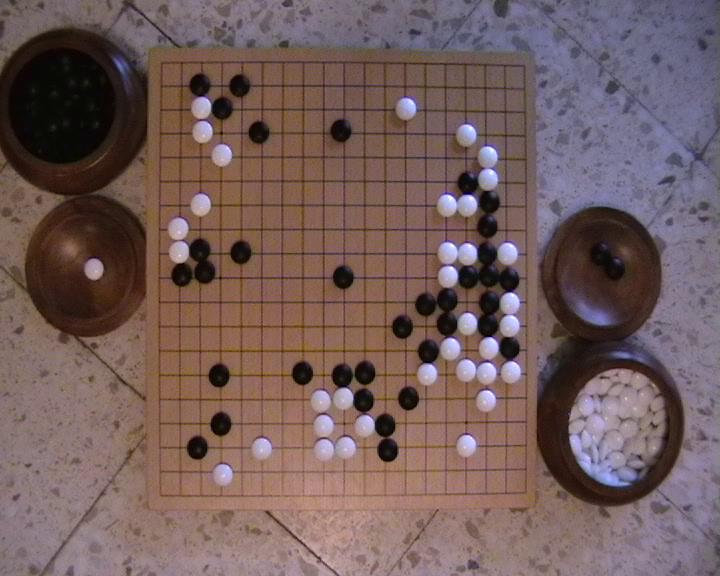
\includegraphics[scale=0.50]{baduk.png}

El go es un juego de mesa estratégico por turnos para dos jugadores. Es 
también conocido como igo (japonés), weiqi (chino) o baduk (coreano). El go 
es notable por ser rico en complejas estrategias a pesar de sus simples reglas.

El juego se realiza por dos jugadores que alternativamente colocan piedras
blancas y negras sobre las intersecciones libres de una cuadrícula de 19x19
líneas. El objetivo del juego es controlar una porción más grande del tablero
que el oponente. Una piedra o grupo de piedras se captura y retira del juego si
no tiene intersecciones vacías adyacentes, esto es, si se encuentra
completamente rodeada de piedras del color contrario.

Ubicar piedras juntas ayuda a protegerlas entre sí y evitar ser capturadas. Por
otro lado, colocarlas separadas hace que se tenga influencia sobre una mayor
porción del tablero. Parte de la dificultad estratégica del juego surge a la
hora de encontrar un equilibrio entre estas dos alternativas. Los jugadores
luchan tanto de manera ofensiva como defensiva y deben elegir entre tácticas de
urgencia y planes a largo plazo más estratégicos.

El go se originó en China hace más de 2 500 años y aunque no se sabe con
exactitud cuándo fue inventado, hacia el 300 a.C. era ya un pasatiempo popular,
como viene indicado en una referencia al juego en Los Analectas de Confucio.
Restos arqueológicos muestran que este antiguo juego se practicaba en un tablero de
una cuadrícula de 17 x 17, pero en la época en la que el juego ya había llegado
a Corea y Japón, sobre el Siglo VII, los tableros habituales eran ya de 19 x 19.

El juego es muy popular en Asia Oriental, pero recientemente ha ganado cierta
popularidad en otras partes del mundo. El go llegó a Europa a través de Japón,
por ello es más conocido internacionalmente por su nombre japonés.


\subsection{¿Qué es un archivo .sgf?, para qué sirve y como podemos abrirlo}

\label{sgf} Un archivo .sgf es un archivo donde se guarda una partida de
go. Como el formato es usado también para muchos juegos de tablero, está
bastante extendido y casi todos los programas de go lo soportan.

El archivo .sgf nos sirve para comentar una partida y hacer pruebas directamente
desde un programa. Otro de los muchos
usos que tiene es guardar todas las partidas para poder verlas en un futuro sin
ocupar apenas espacio en el disco. 

Algunos programas que existen para abrir los .sgf pueden ser, por ejemplo,
quarry, qgo o CGoban. Podemos ver más abajo una imagen del programa quarry. No
solo sirven para abrir .sgf, suelen también servir para jugar en servidores o
contra una IA. Aprovechamos que hemos hablado de IA para comentar que no existe
en la actualidad una IA capaz de ganar a ningún profesional del go.

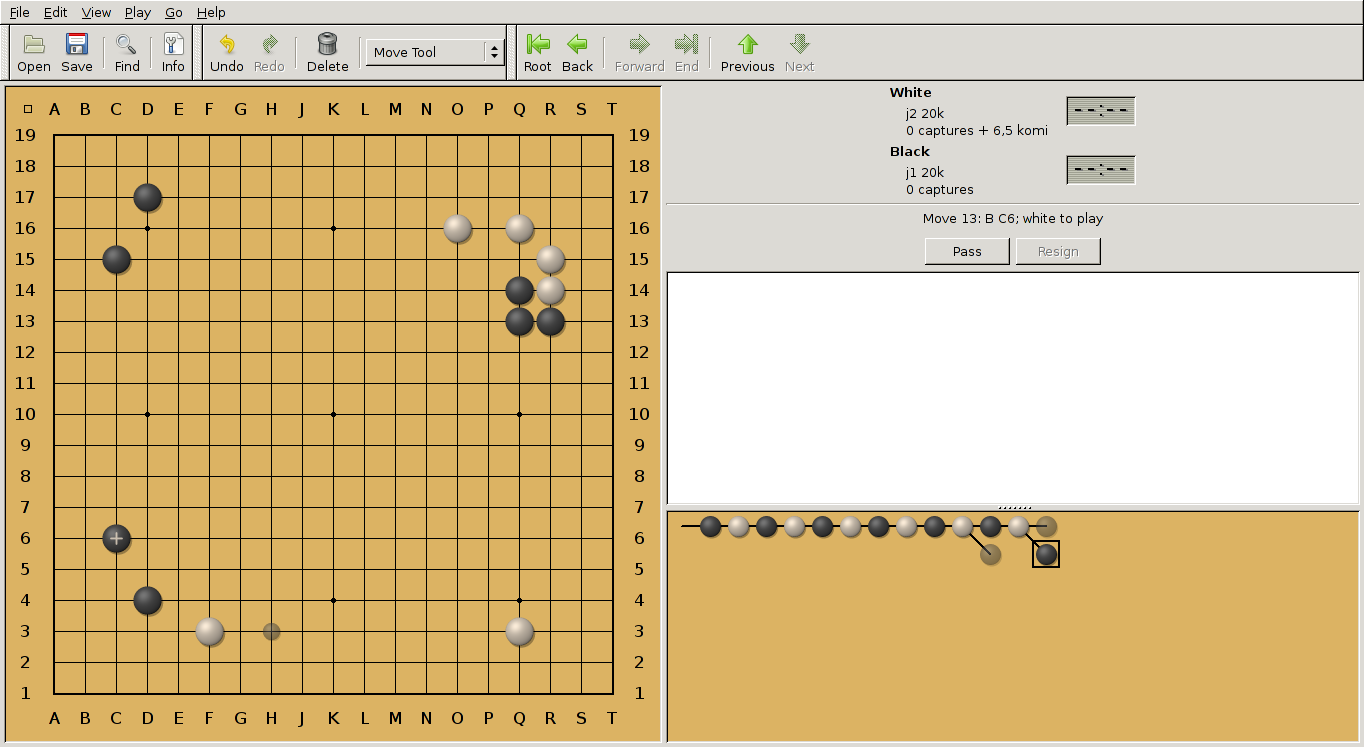
\includegraphics[scale=0.33]{quarry.png}

\chapter{Hardware}

\section{Robot industrial}

\subsection{Introducción}

Existen ciertas dificultades a la hora de establecer una definición formal de lo
que es un robot industrial. 

La primera de ellas surge de la diferencia
conceptual entre el mercado japonés y el euro-americano de lo que es un robot y
lo que es un manipulador. Así, mientras que para los japoneses un robot
industrial es cualquier dispositivo mecánico dotado de articulaciones móviles
destinado a la manipulación, el mercado occidental es más restrictivo, exigiendo
una mayor complejidad, sobre todo en lo relativo al control. 

En segundo lugar, y centrándose ya en el concepto occidental, aunque existe una
idea común acerca de lo que es un robot industrial, no es fácil ponerse de
acuerdo a la hora de establecer una definición formal. Además, la evolución de
la robótica ha ido obligando a diferentes actualizaciones de su definición.

La definición más comúnmente aceptada posiblemente sea la de la Asociación de
Industrias Robóticas (RIA), según la cual:

\emph{Un robot industrial es un manipulador multifuncional reprogramable, capaz de
mover materias, piezas, herramientas, o dispositivos especiales, según
trayectorias variables, programadas para realizar tareas diversas.}

Esta definición, ligeramente modificada, ha sido adoptada por la Organización
Internacional de Estándares (ISO) que define al robot industrial como:

\emph{Manipulador multifuncional reprogramable con varios grados de libertad, capaz de
manipular materias, piezas, herramientas o dispositivos especiales según
trayectorias variables programadas para realizar tareas diversas.}

Se incluye en esta definición la necesidad de que el robot tenga varios grados
de libertad. Una definición más completa es la establecida por la Asociación
Francesa de Normalización (AFNOR), que define primero el manipulador y,
basándose en dicha definición, el robot:

\emph{Manipulador: mecanismo formado generalmente por elementos en serie, articulados
entre sí, destinado al agarre y desplazamiento de objetos. Es multifuncional y
puede ser gobernado directamente por un operador humano o mediante dispositivo
lógico.}

\emph{Robot: manipulador automático servo-controlado, reprogramable, polivalente,
capaz de posicionar y orientar piezas, útiles o dispositivos especiales,
siguiendo trayectoria variables reprogramables, para la ejecución de tareas
variadas. Normalmente tiene la forma de uno o varios brazos terminados en una
muñeca. Su unidad de control incluye un dispositivo de memoria y ocasionalmente
de percepción del entorno. Normalmente su uso es el de realizar una tarea de
manera cíclica, pudiéndose adaptar a otra sin cambios permanentes en su
material.}

Por último, la Federación Internacional de Robótica (IFR) distingue entre robot
industrial de manipulación y otros robots:

\emph{Por robot industrial de manipulación se entiende una máquina de manipulación
automática, reprogramable y multifuncional con tres o más ejes que pueden
posicionar y orientar materias, piezas, herramientas o dispositivos especiales
para la ejecución de trabajos diversos en las diferentes etapas de la producción
industrial, ya sea en una posición fija o en movimiento.}

En esta definición se debe entender que la reprogramabilidad y la multifunción
se consiguen sin modificaciones físicas del robot.

Común en todas las definiciones anteriores es la aceptación del robot industrial
como un brazo mecánico con capacidad de manipulación y que incorpora un control
más o menos complejo. Un sistema robotizado, en cambio, es un concepto más
amplio. Engloba todos aquellos dispositivos que realizan tareas de forma
automática en sustitución de un ser humano y que pueden incorporar o no a uno
o varios robots, siendo esto último lo más frecuente.

\subsection{Historia}

George Charles Devol fue el fundador del primer robot industrial.
Además, junto a Joseph F. Engelberger fundó Unimation, la primera empresa de
robótica de la historia.

Debido a la fusión de la creatividad de Devol y las dotes comerciales de
Engelberger, consiguieron en 1960 un contrato con la General Motors para
instalar un brazo robótico, el Unimate, en su fábrica de Trenton (Nueva Jersey).
La máquina, con un peso de 1.800 kg, fue considerada el primer robot industrial
de la historia y su función era la de levantar y apilar grandes piezas de metal
caliente.

En 1968, Engelberger visitó Japón y consiguió firmar acuerdos con Kawasaki para
la construcción de robots del tipo Unimate. El crecimiento de la robótica en
Japón tuvo como consecuencia directa que Japón adelantara a Estados Unidos
gracias a Nissan, que formó la primera asociación robótica del mundo: la
Asociación Robótica Industrial de Japón (JIRA) en 1972. 

En 1973 KUKA construyó su primer robot industrial, conocido como FAMULUS. Se
trataba del primer robot del mundo con seis ejes de accionamiento
electromecánico.

En 1974 tuvo lugar la creación del Instituto de
Robótica de América (RIA).

En 1978, el primer robot programable de Devol se transformaría en el robot PUMA
(Programmable Universal Machine for Assembly), inventado por Víctor Scheinman. El PUMA era capaz de mover un
objeto y colocarlo en cualquier orientación en un lugar deseado que estuviera a
su alcance. El concepto básico multiarticulado del PUMA es la base de la mayoría
de los robots actuales.

En 1980 se fundó la Federación Internacional de Robótica con sede en Suecia.
En la actualidad, la mayoría de robots están destinados a un uso industrial para
labores como el ensamblaje, soldadura y desplazamiento de materiales.

\subsection{Clasificación del robot industrial}

En general, los robots no tienen clasificación estandarizada, dependiendo de
algunas características se podrían clasifican de distinta forma. Una de las
formas en la que podemos clasificarlos, sería la siguiente: 
\begin{itemize}
    \item Robots manipuladores
    Son sistemas mecánicos multifuncionales, con un sencillo sistema de control,
    que permite gobernar el movimiento de sus elementos, de modo manual o de
    secuencia(fija o variable).  Estos dispositivos suelen emplearse cuando las
    funciones de trabajo son sencillas y repetitivas.
    \item Robots de aprendizaje o repetición
    Son manipuladores que se limitan a repetir una secuencia de movimientos,
    previamente ejecutada por un operador humano, haciendo uso de un
    controlador manual o un dispositivo auxiliar. Programación gestual. 
    Estos robots son los más conocidos hoy día.
    \item Robot de ordenadores
    Son manipuladores o sistemas mecánicos multifuncionales, controlados por un
    ordenador, que habitualmente suele ser un microordenador. Programación textual. 
    Ofrece grandes ventajas y exigen personal cualificado capaz de desarrollar
    programas similares a los de tipo informático.
    \item Robots inteligentes
    Similares a los anteriores, pero además son capaces de relacionarse con el mundo
    que les rodea a través de sensores y tomar decisiones en tiempo real (auto
    programable).
    Son poco conocidos y están en fase experimental. 
    De momento, son muy poco conocidos en el mercado
    \item Micro-robots
    Con fines educacionales, de entretenimiento o investigación, existen numerosos
    robots de formación o micro-robots a un precio muy asequible y, cuya estructura
    y funcionamiento son similares a los de aplicación industrial.
\end{itemize}


\subsection{Componentes}

Los componentes que forman parte de la totalidad del robot son:

\begin{itemize}
    \item Manipulador
    \item Controlador
    \item Dispositivos de entrada y salida de datos
    \item Dispositivos especiales
\end{itemize}


\subsubsection{Manipulador}

Mecánicamente, es el componente principal. Está formado por una serie de
elementos estructurales sólidos o eslabones unidos mediante articulaciones
que permiten un movimiento relativo entre cada dos eslabones consecutivos. 

Las partes que conforman el manipulador son el cuerpo, el brazo, la muñeca y el
actuador final. 

Cada articulación provee al robot de un grado de libertad como mínimo. En
otras palabras, las articulaciones permiten al manipulador realizar
movimientos lineales o angulares. Existen dos tipos, lineal y rotacional. 

La orientación de un eslabón del manipulador se determina
mediante los elementos roll, pitch y yaw.

A la muñeca de un manipulador le corresponden los movimientos o grados de
libertad siguientes: giro, elevación y desviación. No todas las muñecas pueden
realizar estos 3 movimientos. 

El actuador final es un dispositivo que se une a la muñeca del
brazo del robot con la finalidad de activarlo para la realización de una
tarea específica. Existen distintos tipos de elementos
terminales para realizar diferentes funcionalidades. Los diversos
tipos podemos dividirlos en dos grandes categorías: pinzas y herramientas.


\subsubsection{Controlador}
Es el que regula cada uno de los movimientos del manipulador, las acciones,
cálculos y procesado de la información. El controlador recibe y envía señales a
otras máquinas-herramientas y almacena programas.

Existen varios grados de control en función del tipo de
parámetros que se regulan, lo que da lugar a los siguientes tipos de
controladores:
\begin{itemize}
    \item De posición:
    El controlador interviene únicamente en el control de la posición del
    elemento terminal.
    \item Cinemático: 
    En este caso el control se realiza sobre la posición y la velocidad.
    \item Dinámico:
    Además de regular la velocidad y la posición, controla las propiedades
    dinámicas del manipulador y de los elementos asociados a él.
    \item Adaptativo: 
    Engloba todas las regulaciones anteriores y, además, se ocupa de controlar 
    la variación de las características del manipulador al variar la posición.
\end{itemize}


\subsubsection{Dispositivos de entrada y salida}
Los más comunes son: teclado, monitor y caja de comandos.

Los dispositivos de entrada y salida permiten introducir y, a su vez, ver los
datos del controlador. Para mandar instrucciones al controlador y para dar de
alta programas de control, comúnmente se utiliza un ordenador adicional. Es
necesario aclarar que algunos robots únicamente poseen uno de estos componentes.
En estos casos, uno de los componentes de entrada y salida permite la
realización de todas las funciones.

Las señales de entrada y salida se obtienen mediante tarjetas electrónicas
instaladas en el controlador del robot las cuales le permiten tener comunicación
con otras máquinas-herramientas


\subsubsection{Dispositivos especiales}
Entre estos se encuentran los ejes que facilitan el movimiento transversal del
manipulador y las estaciones de ensamblaje, que son utilizadas para sujetar las
distintas piezas de trabajo.



\subsection{Características principales}

Las características más relevantes de los robots podríamos decir que son las
siguientes:

\begin{itemize}
    \item Grados de libertad
    \item Volumen de trabajo
    \item Precisión de los movimientos
    \item Capacidad de carga
    \item Velocidad
    \item Tipo de actuadores
    \item Programabilidad
\end{itemize}
 

    
\subsubsection{Grados de libertad}

Son cada uno de los movimientos independientes que
puede realizar cada articulación con respecto a la anterior. Son los
parámetros que se precisan para determinar la posición y la orientación del
elemento terminal del manipulador. El número de grados de libertad del robot
viene dado por la suma de los grados de libertad de las articulaciones que lo componen.
Puesto que las articulaciones empleadas suelen ser únicamente de rotación y
lineal, con un solo grado de libertad cada una, el número de grados de libertad del
robot suele coincidir con el número de articulaciones que lo componen. 

Puesto que para posicionar y orientar un cuerpo de cualquier manera en el
espacio son necesarios seis parámetros, tres para definir la posición y tres
para la orientación, si se pretende que un robot posicione y oriente su
extremo (y con él la pieza o herramienta manipulada) de cualquier modo en el
espacio, se precisará al menos seis grados de libertad.

Un mayor número de grados de libertad conlleva un aumento de la flexibilidad
en el posicionamiento del elemento terminal. Aunque la mayoría de las
aplicaciones industriales requieren 6 grados de libertad, como las de la soldadura,
mecanizado y paletización, otras más complejas requieren un número mayor,
como es el caso en las labores de montaje. Si se trabaja en un entorno con
obstáculos, el dotar al robot de grados de libertad adicionales le permitirá
acceder a posiciones y orientaciones de su extremo a las que, como
consecuencia de los obstáculos, no hubieran llegado con seis grados de
libertad. Otra situación frecuente es dotar al robot de un grado de libertad
adicional que le permita desplazarse a lo largo de un carril aumentando así
el volumen del espacio al que puede acceder. Tareas más sencillas y con
movimientos más limitados, como las de la pintura y paletización, suelen
exigir 4 o 5 grados de libertad.

Observando los movimientos del brazo y de la muñeca, podemos determinar el
número de grados de libertad que presenta un robot. Generalmente, tanto en
el brazo como en la muñeca, se encuentran desde 1 hasta 3 grados de libertad. 


\subsubsection{Volumen de trabajo}

Las dimensiones de los elementos del manipulador, junto a los grados de
libertad, definen la zona de trabajo del robot, característica fundamental en
las fases de selección e implantación del modelo adecuado.

La zona de trabajo se subdivide en áreas diferenciadas entre sí, dependiendo de
la accesibilidad del elemento terminal.

El volumen de trabajo de un robot se refiere únicamente al espacio dentro del
cual puede desplazarse el extremo de su muñeca. Para determinar el volumen de
trabajo no se toma en cuenta el actuador final. La razón de ello es que a la
muñeca del robot se le pueden adaptar actuadores finales diferentes.

Vamos a diferenciar 3 tipos:
\begin{itemize}
    \item El robot cartesiano y el robot cilíndrico presentan volúmenes de
    trabajo regulares, generando una figura cúbica.
    \item El robot de configuración cilíndrica presenta un volumen de trabajo
    parecido a un cilindro.
    \item Los robots que poseen una configuración polar, los de brazo articulado
    y los modelos SCARA presentan un volumen de trabajo irregular. Para
    determinar el volumen de trabajo de un robot industrial, el fabricante
    generalmente indica un plano con los límites de movimiento que tiene cada
    una de las articulaciones del robot.
\end{itemize}


\subsubsection{Precisión de los movimientos}

La precisión de movimiento en un robot industrial depende de tres factores:

\begin{itemize}
    \item Resolución espacial, es el incremento más pequeño de movimiento en que
    el robot puede dividir su volumen de trabajo. 
    \item Exactitud, es la capacidad de un robot para situar el extremo de su
    muñeca en un punto señalado dentro del volumen de trabajo.
    \item Repetibilidad, es la capacidad del robot de regresar al punto
    programado las veces que sean necesarias. 
\end{itemize}


\subsubsection{Capacidad de carga}

Es el peso en kilográmos que puede transportar la garra del manipulador. A
veces, este peso incluye el peso de la propia garra. Esta capacidad, en este
tipo de robots, suele oscilar entre 0.9 y 205 Kg. 

La capacidad de carga es una de las características que más se tienen en
cuenta en la selección de un robot, según la tarea a la que se destine. En
soldadura y mecanizado es común precisar capacidades de carga superiores a los
50kg.


\subsubsection{Velocidad}

Se refiere a la velocidad máxima alcanzable por el punto de centro de la
herramienta o por las articulaciones.
En muchas ocasiones, una velocidad de trabajo elevada, aumenta
extraordinariamente el rendimiento del robot, por lo que esta magnitud se valora
considerablemente en la elección del mismo. En tareas de soldadura y
manipulación de piezas es muy aconsejable que la velocidad de trabajo sea alta.
En pintura, mecanizado y ensamblaje, la velocidad debe ser media e incluso baja.


\subsubsection{Tipo de actuadores}

Los elementos motrices que generan el movimiento de las articulaciones pueden
ser, según la energía que consuma, de los siguientes tipos:

\begin{itemize}
    \item Los actuadores de tipo olehidráulico se destinan a tareas que requieren una gran
    potencia y grandes capacidades de carga. Dado el tipo de energía que emplean, se
    construyen con mecánica de precisión y su coste es elevado. Los robots
    hidráulicos se diseñan formando un conjunto compacto: la central hidráulica, la
    cabina electrónica de control y el brazo del manipulador.
    \item La energía neumática dota a sus actuadores de una gran velocidad de respuesta
    junto a un bajo coste, pero su empleo está siendo sustituido por elementos
    eléctricos.
    \item Los motores eléctricos, que cubren la gama de media y baja potencia, acaparan el
    campo de la Robótica, por su gran precisión en el control de su movimiento y las
    ventajas inherentes a la energía eléctrica que consumen.
\end{itemize}


\subsubsection{Programabilidad}

La inclusión del controlador de tipo microelectrónica en los robots
industriales, permite la programación del robot de muy diversas formas.

En general, los modernos sistemas de robots admiten la programación manual,
mediante un modulo de programación. Las programaciones gestual y textual,
controlan diversos aspectos del funcionamiento del manipulador:

\begin{itemize}
    \item Control de la velocidad y la aceleración.  
    \item Saltos de programas condicionales.  
    \item Temporizaciones y pausas.  
    \item Edición, modificación, depuración y ampliación de programas.  
    \item Funciones de seguridad.  
    \item Funciones de sincronización con otras maquinas.  
    \item Uso de lenguajes específicos de Robótica.
\end{itemize}


\subsection{Selección de robot industrial}

\begin{itemize}
    \item El tipo de nuestro robot debe de ser con control por ordenador, ya
    que necesitamos programar hacia donde queremos que vaya en cada momento, sin
    tener que pulsar botones manualmente. 
    \item Los grados de libertad tenemos suficiente con 6, como suelen ser los
    más típicos. 
    \item El volumen de trabajo buscado es aproximadamente de 0,50 metros
    cúbicos, por lo tanto, podríamos buscar un robot cartesiano o uno de
    configuración polar. Nosotros descartamos el cartesiano porque las
    dimensiones de este para estar fuera del tablero y no estorbar tenían que
    ser muy grandes, por lo tanto, buscamos un robot con configuración polar que
    llegue al menos a una distancia de 0,5 metros. 
    \item Respecto a la precisión de este robot, tenemos que buscar uno que
    tenga bastante, ya que las piedras en una partida de go se encuentran muy
    juntas y una diferencia de pocos milímetros podría entorpecer demasiado. 
    \item Respecto a la capacidad de carga que necesitamos es ínfima, por que
    las piedras de go no pesan mucho. 
    \item Por último, y pensamos que bastante importante, el tipo de actuador para
    coger este robot. Hemos visto bastantes tipos y pensado unos cuantos, pero
    al tener los problemas de que las piedras son convexas por ambos lados y de
    cristal, debemos de tomar mucha precaución a la hora de seleccionar. Quizás
    la mejor elección sean una pinzas con antideslizantes.
    \item Otra de las cosas que buscamos es que no sea muy caro, ya que el
    presupuesto que tenemos no es mucho. 
\end{itemize}


No existe actualmente en el mercado ninguna opción que cumpla todos estos
requisitos, ya que un robot que sea preciso, rápido y un volumen como el que
necesitamos, tienen un precio mayor de los 1000 \euro.

También hemos encontrado un robot que cuesta solamente unos 50-60 \euro, pero es
lento, poco preciso y con un volumen que no llega ni a la mitad del tablero.

Por los motivos anteriormente expresados se llegó a un punto concluyente en el
que se tomó la decisión de no abordar la fase de elaboración del robot.




\section{Arduino}
\subsection{Introducción}
En este proyecto, arduino se utilizará para la creacion del reloj, que indica el
tiempo que le queda a cada jugador, a su vez arduino le indicará al programa
cuando ha terminado el turno de un jugador y cuando ha empezado otro.

También como hemos visto anteriormente, dado a la diversidad de brazos que hay
en el mercado, es muy probable que se use para el manejo del brazo que se usará
para hacer los movimientos físicos.

Arduino es una plataforma de electrónica abierta para la creación de prototipos
basada en software y hardware flexibles y fáciles de usar. Se creó para
artistas, diseñadores, aficionados y cualquiera interesado en crear entornos u
objetos interactivos.

Arduino puede tomar información del entorno a través de sus pines de entrada de
toda una gama de sensores y puede afectar a aquello que le rodea controlando
luces, motores y otros actuadores. El microcontrolador en la placa Arduino se
programa mediante el lenguaje de programación Arduino (basado en Wiring) y el
entorno de desarrollo Arduino (basado en Processing). Los proyectos hechos con
Arduino pueden ejecutarse sin necesidad de conectar a un ordenador, si bien
tienen la posibilidad de hacerlo y comunicar con diferentes tipos de software
(p.ej. Flash, Processing, MaxMSP).

Las placas pueden ser hechas a mano o compradas montadas de fábrica; el software
puede ser descargado de forma gratuita. Los ficheros de diseño de referencia
(CAD) están disponibles bajo una licencia abierta, así pues, eres libre de
adaptarlos a sus necesidades.
Arduino recibió una Mención Honorífica en la sección Digital Communities de la
edición del 2006 del Ars Electronica Prix. El equipo Arduino (Arduino team) es:
Massimo Banzi, David Cuartielles, Tom Igoe, Gianluca Martino, and David Mellis.

\subsection{¿Que es Arduino?}

Arduino es una herramienta para hacer que los ordenadores puedan sentir y
controlar el mundo físico a través de tu ordenador personal. Es una plataforma
de desarrollo de computación física (physical computing) de código abierto,
basada en una placa con un sencillo microcontrolador y un entorno de desarrollo
para crear software (programas) para la placa.

Puedes usar Arduino para crear objetos interactivos, leyendo datos de una gran
variedad de interruptores y sensores y controlar multitud de tipos de luces,
motores y otros actuadores físicos. Los proyecto de Arduino pueden ser autónomos
o comunicarse con un programa (software) que se ejecute en tu ordenador (ej.
Flash, Processing, MaxMSP). La placa puedes montarla tu mismo o comprarla ya
lista para usar, y el software de desarrollo es abierto y lo puedes descargar
gratis.

El lenguaje de programación de Arduino es una implementación de Wiring, una
plataforma de computación física parecida, que a su vez se basa en Processing,
un entorno de programación multimedia.


\subsection{Ventajas de usar Arduino}

Hay muchos otros microcontroladores y plataformas con microcontroladores
disponibles para la computación física. Parallax Basic Stamp, BX-24 de Netmedia,
Phidgets, Handyboard del MIT, y muchos otros ofrecen funcionalidades similares.
Todas estas herramientas organizan el complicado trabajo de programar un
microcontrolador en paquetes fáciles de usar.

Arduino, además de simplificar el proceso de trabajar con microcontroladores,
ofrece algunas ventajas respecto a otros sistemas a profesores, estudiantes y
amateurs:

\begin{itemize} 
    \item Asequible - Las placas Arduino son más asequibles comparadas con
    otras plataformas de microcontroladores. La versión más cara de un modulo
    de Arduino puede ser montada a mano, e incluso ya montada cuesta bastante
    menos de 60 Euros
    
    \item Multi-Plataforma - El software de Arduino funciona en los sistemas
    operativos Windows, Macintosh OSX y Linux. La mayoría de los entornos para
    microcontroladores están limitados a Windows.
    Entorno de programación simple y directo - El entorno de programación de Arduino
    es fácil de usar para principiantes y lo suficientemente flexible para los
    usuarios avanzados. Pensando en los profesores, Arduino está basado en el
    entorno de programación de Procesing con lo que el estudiante que aprenda a
    programar en este entorno se sentirá familiarizado con el entorno de desarrollo
    Arduino.

    \item Software ampliable y de código abierto- El software Arduino esta
    publicado bajo una licencia libre y preparado para ser ampliado por
    programadores experimentados. El lenguaje puede ampliarse a través de
    bibliotecas de C++, y si se está interesado en profundizar en los detalles
    técnicos, se puede dar el salto a la programación en el lenguaje AVR C en el
    que está basado. De igual modo se puede añadir directamente código en AVR C
    en tus programas si así lo deseas.
	
    \item Hardware ampliable y de Código abierto - Arduino está basado en los
    microcontroladores ATMEGA168, ATMEGA328 y ATMEGA1280. Los planos de los
    módulos están publicados bajo licencia Creative Commons, por lo que
    diseñadores de circuitos con experiencia pueden hacer su propia versión del
    módulo, ampliándolo u optimizándolo. Incluso usuarios relativamente
    inexpertos pueden construir la versión para placa de desarrollo para
    entender cómo funciona y ahorrar algo de dinero.
\end{itemize}


\subsection{Modelos}

\subsubsection{Arduino Duemilanove}

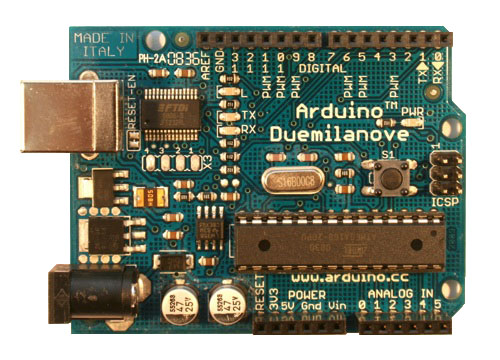
\includegraphics[scale=0.5]{ArduinoDuemilanove.jpg}

Esta es la ultima revisión de la placa Arduino USB básica. Se conecta al
ordenador con un cable USB estándar y contiene todo lo necesario para programar
la placa. Se puede ampliar con gran variedad de shields: placas de extensión con
funcionalidades especificas.


\begin{tabular}{||l | l ||}
\hline
\hline
Microcontrolador & ATmega368 (ATmega168 en versiones anteriores)\\
\hline
Voltaje de funcionamiento & 5V\\
\hline
Voltaje de entrada (recomendado) & 7-12V\\
\hline
Voltaje de entrada (limite) & 6-20V\\
\hline
Pines E/S digitales & 14 (6 proporcionan salida PWM)\\
\hline
Pines de entrada analógica & 6\\
\hline
Intensidad por pin & 40 mA\\
\hline
Intensidad en pin & 3.3V	50 mA\\
\hline
Memoria Flash & 16 KB (ATmega168)\\
\hline
Memoria Flash & 32 KB (ATmega328)\\
\hline
SRAM & 1 KB (ATmega168)\\
\hline
SRAM & 2 KB (ATmega328)\\
\hline
EEPROM & 512 bytes (ATmega168)\\
\hline
EEPROM & 1 KB (ATmega328)\\
\hline
Velocidad de reloj & 16 MHz\\
\hline
\hline
\end{tabular}

\subsubsection{Arduino Diecimila}

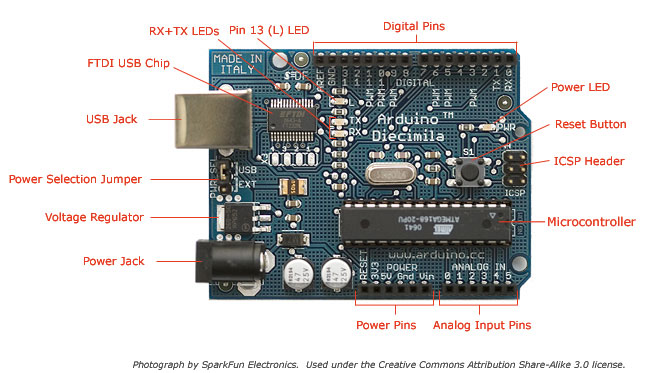
\includegraphics[scale=0.6]{ArduinoDiecimilaComponents.jpg}

 Esta es la revisión anterior de la placa USB básica.

\begin{tabular}{||l | l ||}
\hline
\hline
Microcontrolador & ATmega168\\
\hline
Voltaje de funcionamiento & 5V\\
\hline
Voltaje de entrada (recomendado) & 7-12 V\\
\hline
Voltaje de entrada (limites) & 6-20 V\\
\hline
Pines E/S Digitales & 14 (de ellos 6 son salidas PWM)\\
\hline
Pines de entrada Analógica & 6\\
\hline
Intensidad por pin de E/S & 40 mA\\
\hline
Intensidad por pin de 3.3V & 50 mA\\
\hline
Memoria Flash & 16 KB (2 KB reservados para el gestor de arranque)\\
\hline
SRAM & 1 KB\\
\hline
EEPROM & 512 bytes\\
\hline
Velocidad del reloj & 16 MHz\\
\hline
\hline
\end{tabular}

\subsubsection{Nano}

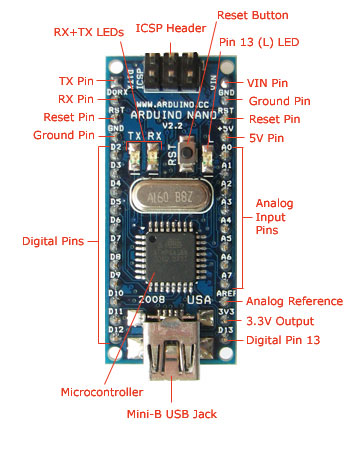
\includegraphics[scale=0.6]{NanoFront.jpg}

El Arduino Nano es una pequeña y completa placa basada en el ATmega328 (Arduino
Nano 3.0) o ATmega168 (Arduino Nano 2.x) que se usa conectándola a una
protoboard. Tiene más o menos la misma funcionalidad que el Arduino Duemilanove,
pero con una presentación diferente. No posee conector para alimentación
externa, y funciona con un cable USB Mini-B en vez de el cable estandar. El nano
fue diseñado y está siendo producido por Gravitech.

\begin{tabular}{||l | l ||}
\hline
\hline
Microcontrolador & Atmel ATmega168 o ATmega328\\
\hline
Tensión de Operación (nivel lógico) & 5 V\\
\hline
Tensión de Entrada (recomendado) & 7-12 V\\
\hline
Tensión de Entrada (límites) & 6-20 V\\
\hline
Pines E/S Digitales & 14 (de los cuales 6 proveen de salida PWM\\
\hline
Entradas Analógicas & 8\\
\hline
Corriente máx por cada PIN de E/S & 40 mA\\
\hline
Memoria Flash & 16 KB (ATmega168)\\
\hline
SRAM & 1 KB (ATmega168)\\
\hline
EEPROM & 512 bytes (ATmega168)\\
\hline
Frecuencia de reloj & 16 MHz\\
\hline
Dimensiones & 18,5mm x 43.2mm\\
\hline
\hline
\end{tabular}

\subsubsection{Arduino Mega}

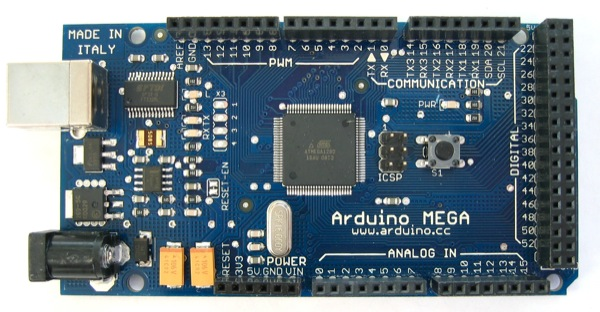
\includegraphics[scale=0.6]{ArduinoMega.jpg}

El Arduino Mega es una placa microcontrolador basada ATmeg1280 (datasheet). Tiene 54 entradas/salidas digitales (de las cuales 14 proporcionan salida PWM), 16 entradas digitales, 4 UARTS (puertos serie por hardware), un cristal oscilador de 16MHz, conexión USB, entrada de corriente, conector ICSP y botón de reset. Contiene todo lo necesario para hacer funcionar el microcontrolador; simplemente conectálo al ordenador con el cable USB o aliméntalo con un trasformador o batería para empezar. El Mega es compatible con la mayoría de shields diseñados para el Arduino Duemilanove o Diecimila

\subsubsection{Arduino Bluetooth}

El Arduino BT contiene un modulo bluetooth que permite comunicarse y programarse
sin cables. Es compatible con los shields de Arduino. 
El módulo Bluetooth utilizado es el Bluegiga WT11, la versión iWrap. El módulo
Bluetooth se puede configurar con comandos enviados a través del puerto serie
del ATmega168. Un programa para configurar el nombre y código del módulo
bluetooth se ejecuta una vez en cada BT Arduino. El nombre se establece en
ARDUINOBT y el código de acceso en 12345. Para obtener detalles más completos,
ve al código fuente del programa Initialization. El ATmega168 viene precargado
con un gestor de arranque que te permite subir sketches al consejo de
administración a través de bluetooth. El código fuente del gestor de arranque
está disponible en el repositorio SVN de Arduino.

\subsubsection{Arduino LilyPad}

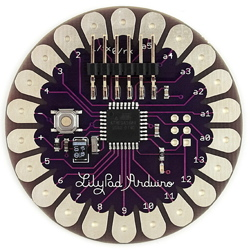
\includegraphics[scale=0.6]{LilyPad_3.jpg}

Diseñado para aplicaciones sobre prendas, esta placa puede ser cosida a la ropa
y es de color purpura y con un diseño con estilo. 

\begin{tabular}{||l | l ||}
\hline
\hline
Microcontrolador & ATmega168V o ATmega328V\\
\hline
Voltaje de funcionamiento & 2.7-5.5 V\\
\hline
Voltaje de entrada & 2.7-5.5 V\\
\hline
Pines E/S Digitales & 14 (de las cuales 6 proporcionan salida PWM)\\
\hline
Pines Entradas Analógicas Input Pins & 6\\
\hline
Intensidad por pin & 40 mA\\
\hline
Memora Flash & 16 KB \\
\hline
SRAM & 1 KB\\
\hline
EEPROM & 512 bytes\\
\hline
Velocidad de reloj & 8 MHz\\
\hline
\hline
\end{tabular}


\subsubsection{Arduino Fio}

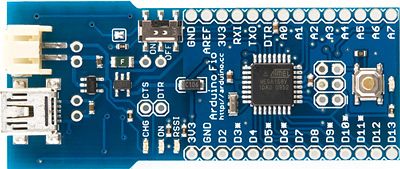
\includegraphics[scale=0.6]{ArduinoFio.jpg}

Diseñada para aplicaciones inalámbricas. Incluye un zócalo para XBee, un
conector para baterías LiPo y electrónica para cargar baterías. 

\begin{tabular}{||l | l ||}
\hline
\hline
Microcontrolador & ATmega328P\\
\hline
Voltaje de trabajo & 3.3V\\
\hline
Voltaje de Entrada & 3.35 -12 V\\
\hline
Voltaje de Entrada en Carga & 3.7 - 7 V\\
\hline
Pines E/S Digital & 14 (of which 6 provide PWM output)\\
\hline
Pines de Entrada Analógica & 8\\
\hline
Corriente DC por pin E/S & 40 mA\\
\hline
Memoria Flas & 	32 KB (of which 2 KB used by bootloader)\\
\hline
SRAM & 2 KB\\
\hline
EEPROM & 1 KB\\
\hline
Frecuencia de Reloj & 8 MHz\\
\hline
\hline
\end{tabular}

\subsubsection{Arduino Mini}

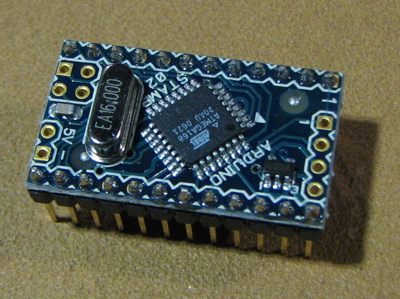
\includegraphics[scale=0.6]{arduino_mini.jpg}

La placa Arduino más pequeña. Funciona perfectamente en una placa de desarrollo
o en aplicaciones donde el espacio es primordial. Se conecta al ordenador usando
el adaptador Mini USB. 

\begin{tabular}{||l | l ||}
\hline
\hline
Microcontrolador & ATmega168\\
\hline
Voltaje de funcionamiento & 5V\\
\hline
Voltaje de entrada & 7-9 V\\
\hline
Pines E/S digital & 14 (6 pueden ser usadas como salidas PWM)\\
\hline
Pines entrada analógica & 8 (de las cuales 4 se extienden en pines)\\
\hline
DC Corriente continua por pin E/S & 40 mA\\
\hline
Memoria Flash & 16 KB (de las cuales 2 KB son usadas por el bootloader)\\
\hline
SRAM & 1 KB\\
\hline
EEPROM & 512 bytes\\
\hline
Velocidad de reloj & 16 MHz\\
\hline
\hline
\end{tabular}

\subsubsection{Arduino Adaptador Mini USB}

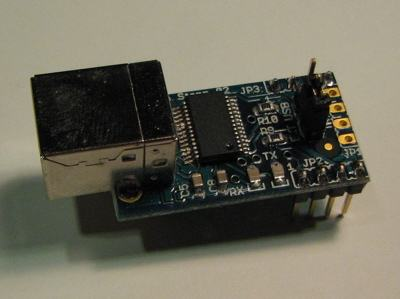
\includegraphics[scale=0.6]{mini_usb.jpg}

Esta placa convierte una conexión USB a TX y RX de 5 voltios que se puede
conectar directamente al Arduino Mini u otros microcontroladores, permitiéndoles
comunicarse con el ordenador. Se basa en el chip de FTDI FT232RL, (los
controladores se incluyen con el software de Arduino).

\subsubsection{Arduino Pro}

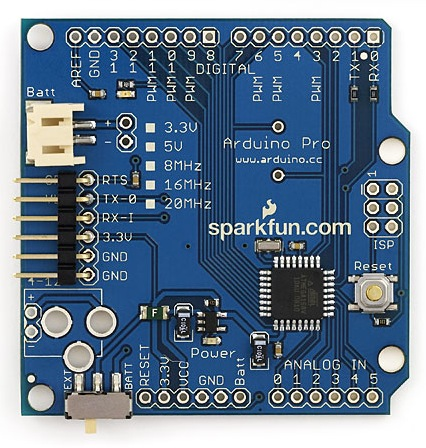
\includegraphics[scale=0.6]{ArduinoPro.jpg}

Esta placa esta diseñada para aquellos que quien dejar la placa incrustada en el
proyecto: es más barata que la Diecimila y se puede alimentar fácilmente con
baterías. pero requiere de componentes extra y montaje. 

\begin{tabular}{||l | l ||}
\hline
\hline
Microcontrolador & ATmega168 o ATmega328\\
\hline
Voltaje de funcionamiento & 3.3v o 5v\\
\hline
Voltaje de entrada & 3.35 -12v o 5 - 12v\\
\hline
Pines digitales de E/S & 14 (6 de los cuales tienen salida PWM)\\
\hline
Pines de entrada analógica & 6\\
\hline
Intensidad máxima por E/S & 40 mAv\\
\hline
Memoria Flash & 16KB en el ATmega168 y 32KB con el ATmega328 \\
\hline
SRAM & 1KB\\
\hline
EEPROM & 512 bytes\\
\hline
Velocidad de Reloj & 8 MHz o 16 MHz\\
\hline
\hline
\end{tabular}

\subsubsection{Arduino Pro Mini}

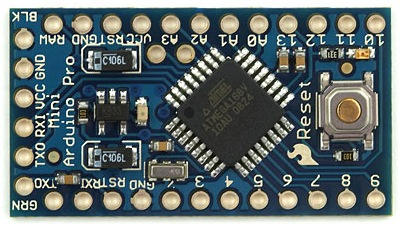
\includegraphics[scale=0.6]{ArduinoProMini.jpg}

Como la Pro, la Pro Mini esta diseñada para usuarios avanzados que requieren de
bajo coste, menor tamaño y dispuestos a un poco de trabajo extra. 

\begin{tabular}{||l | l ||}
\hline
\hline
Microcontrolador & ATmega168\\
\hline
Voltaje de funcionamiento & 3.3v o 5v (dependiento del modelo)\\
\hline
Voltaje de entrada & 3.35 -12v o 5 - 12v\\
\hline
Pines digitales de E/S & 14 (6 de los cuales tienen salida PWM)\\
\hline
Pines de entrada analógica & 6\\
\hline
Intensidad máxima por E/S & 40 mA\\
\hline
Memoria Flash & 16KB\\
\hline
SRAM & 1KB\\
\hline
EEPROM & 512 bytes\\
\hline
Velocidad de Reloj & 8 MHz (modelo de 3.3v) o 16 MHz (modelo de 5v)\\
\hline
\hline
\end{tabular}

\subsubsection{Arduino Serial}

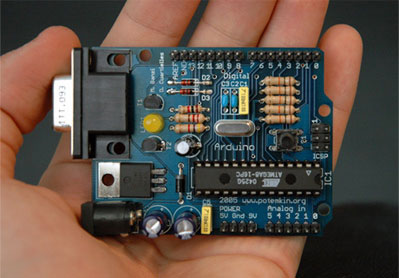
\includegraphics[scale=0.6]{arduino.jpg}

Es una placa básica que utiliza una interfaz RS232 para comunicarse con el
ordenador o para la carga de sketches. Esta placa es fácil de montar, incluso
como ejercicio de aprendizaje. Se ha diseñado para utilizar los componentes más
simples posibles, de manera que sea fácil de construir, incluso si buscas las
componentes en la tienda de la esquina.







\section{Cámaras}
\subsection{Introducción}

Para este proyecto, la cámara es fundamental, ya que esta se encargara de la
captación de imagenes, tanto para la detección del tablero y las piedras del
jugador como para situar correctamente la piedra que queremos colocar en su
sitio.

Debido a que usaremos Opencv para la selección de cámaras, los diferentes
modelos segun la conexion no entran en el ambito de este proyecto, dejando una
clara importancia a la resolución de la imagen, que en gran parte viene dada por
el tipo de lente y el metodo de captación 

La mayor parte de las cámaras digitales se pueden conectar directamente al
ordenador para transferir su información. Antiguamente las cámaras tenían que
conectarse a través de un Puerto serie. El USB es el método más utilizado aunque
algunas cámaras utilizan un puerto FireWire o Bluetooth. La mayor parte de las
cámaras son reconocidas como un dispositivo de almacenamiento USB. Algunos
modelos, por ejemplo la Kodak EasyShare One puede conectarse al ordenador
vía red inalámbrica por el protocolo 802.11 (Wi-Fi).

\subsection{Historia}

Los conceptos de digitalizar imágenes en escaneres y convertir señales de video
a digital anteceden al concepto de tomar cuadros fijos digitalizando así señales
de una matriz de elementos sensores discretos. Eugene F. Lally del Jet
Propulsion Laboratory publicó la primera descripción de cómo producir fotos
fijas en un dominio digital usando un fotosensor en mosaico.2 El propósito era
proporcionar información de navegación a los astronautas a bordo durante
misiones espaciales. La matriz en mosaico registraba periódicamente fotos fijas
de las localizaciones de estrellas y planetas durante el tránsito y cuando se
acercaba a un planeta, proporcionaba información adicional de distancias para el
orbitaje y como guía para el aterrizaje. El concepto incluyó elementos de diseño
que presagiaban la primera cámara fotográfica digital.
Texas Instruments diseñó una cámara fotográfica análoga sin película en 1972,
pero no se sabe si fue finalmente construida. La primera cámara digital
registrada fue desarrollada por la empresa Kodak, que encargó la construcción de
un prototipo al ingeniero Steven J. Sasson en 1975. Esta cámara usaba los
entonces nuevos sensores CCD desarrollados por Fairchild Semiconductor en 1973.
Su trabajo dio como fruto una cámara de aproximadamente 4 kg. y que hacía fotos
en blanco y negro con una resolución de 0,01 megapíxeles. Utilizó los novedosos
chips de estado sólido del CCD. La cámara fotográfica registraba las imágenes en
una cinta de cassette y tardó 23 segundos en capturar su primera imagen, en
diciembre de 1975. Este prototipo de cámara fotográfica era un ejercicio
técnico, no previsto para la producción.
\subsubsection{La verdadera cámara digital }
La primera cámara fotográfica digital verdadera que registraba imágenes en un
archivo de ordenador fue probablemente el modelo DS-1P de Fuji, en 1988, que
grababa en una tarjeta de memoria interna de 16 MB y utilizaba una batería para
mantener los datos en la memoria. Esta cámara fotográfica nunca fue puesta en
venta en los Estados Unidos. La primera cámara fotográfica digital disponible en
el mercado fue la Dycam Model 1, en 1991, que también fue vendida con el nombre
de Logitech Fotoman. Usaba un sensor CCD, grababa digitalmente las imágenes, y
disponía de un cable de conexión para descarga directa en el ordenador.
En 1991, Kodak lanzó al mercado su modelo DCS-100, el primero de una larga línea
de cámaras fotográficas profesionales SLR de Kodak que fueron basadas, en parte,
en cámaras para película, a menudo de marca Nikon. Utilizaba un sensor de 1,3
megapixeles y se vendía en unos 13.000 dolares.
La transición a formatos digitales fue ayudada por la formación de los primeros
estándares JPEG y MPEG en 1988, que permitieron que los archivos de imagen y
vídeo se comprimieran para su almacenamiento. La primera cámara fotográfica
dirigida a consumidores con una pantalla de cristal líquido en la parte
posterior fue la Casio QV-10 en 1995, y la primera cámara fotográfica en
utilizar tarjetas de memoria CompactFlash fue la Kodak DC-25 en 1996.

El mercado para las cámaras fotográficas digitales dirigidas al consumidor
estaba formado originalmente por cámaras fotográficas de baja resolución. En
1997 se ofrecieron las primeras cámaras fotográficas para consumidores de un
megapixel. La primera cámara fotográfica que ofreció la capacidad de registrar
clips de vídeo pudo haber sido la Ricoh RDC-1 en 1995.
En 1999 con la introducción del Nikon D1, una cámara fotográfica de 2.74
megapixeles, que fue una de las primeras SLR digitales, la compañía se convirtió
en un fabricante importante, y, con un costo inicial de menos de 6.000 dolares,
era asequible tanto para fotógrafos profesionales como para consumidores de alto
perfil. Esta cámara fotográfica también utilizaba lentes Nikon F, lo que
significaba que los fotógrafos podrían utilizar muchas de las mismas lentes que
ya tenían para sus cámaras de película.
En el 2003 se presentó la Digital Rebel de Canon, también conocida como la 300D,
una cámara fotográfica dirigida a consumidores de 6 megapixeles y la primera
DSLR que tenía un costo inferior a 1.000 dolares.
En el 2008 se presentó en la Feria de Alemania, una cámara LEICA de medio
formato con una resolución de 37 megapixeles.

\subsubsection{Historia de las Camaras web}

En el Departamento de Informática de la Universidad de Cambridge la cafetera
estaba situada en un sótano. Si alguien quería un café tenía que bajar desde su
despacho y, si lo había, servirse una taza. Si no lo había, tenía que hacerlo.
Las normas decían que el que se termina la cafetera debe rellenarla, pero
siempre había listos que no cumplian con las normas.
En 1991, Quentin Stafford-Fraser y Paul Jardetzky, que compartían despacho,
hartos de bajar tres plantas y encontrarse la cafetera vacía decidieron pasar al
contraataque. Diseñaron un protocolo cliente-servidor que conectándolo a una
cámara, trasmitía una imagen de la cafetera a una resolución de 128 x 128
pixels.
Así, desde la pantalla de su ordenador sabían cuando era el momento propicio
para bajar a por un café, y de paso sabían quienes eran los que se acababan la
cafetera y no la volvían a llenar. El protocolo se llamó XCoffee y tras unos
meses de depuración se decidieron a comercializarlo. En 1992 salió a la venta la
primera cámara web llamada XCam.

\subsection{Resolución}

La resolución de una cámara fotográfica digital está limitada por el sensor de
la cámara (generalmente un CCD o un Sensor CMOS) que responde a las señales de
luz, substituyendo el trabajo de la película en fotografía tradicional. El
sensor se compone de millones de “cubos” que se cargan en respuesta a la luz.
Generalmente, estos cubos responden solamente a una gama limitada de longitudes
de onda ligeras, debido a un filtro del color sobre cada uno. Cada uno de estos
cubos se llama un píxel, y se utiliza un algoritmo de mosaicismo e interpolación
para unir la imagen de cada gama de longitud de onda por pixel en una imagen del
RGB donde están las tres imágenes por píxel para representar un color completo.

Los dispositivos CCD transportan la carga a través del chip hasta un conversor
analógico-digital. Éste convierte el valor de cada uno de los píxeles en un
valor digital midiendo la carga que le llega. Dependiendo del número de bits del
conversor obtendremos una imagen con mayor o menor gama de color. Por ejemplo,
si se utilizase un sólo bit tendríamos valores de 0 y 1, y sólo podríamos
representar presencia o ausencia de luz, lo que supondría una imagen en blanco y
negro puro.

Por otro lado, los aparatos CMOS contienen varios transistores en cada píxel. El
proceso de conversión digital se produce en la propia estructura del sensor, por
lo que no se necesita un conversor añadido. Su proceso de fabricación es más
sencillo, y hace que las cámaras que utilizan esta tecnología resulten más
baratas.

La cantidad de pixeles resultante en la imagen determina su tamaño. Por ejemplo
una imagen de 640 pixeles de ancho por 480 pixeles de alto tendrá 307,200
pixels, o aproximadamente 307 kilopixeles; una imagen de 3872 pixeles de alto
por 2592 pixeles de ancho tendrá 10.036.224 pixeles, o aproximadamente 10
megapixeles.

Según la experiencia fotográfica de los profesionales en dicho campo afirman que
una fotografía química realizada por una cámara compacta daría como resultado
una fotografía de 30 megapixeles.

\subsection{Lentes}

La lente de la cámara enfoca la imagen en el sensor de imagen
(CCD). Antes de llegar al sensor la imagen pasa por el filtro óptico que
elimina cualquier luz infrarroja de forma que se muestren los colores
correctos, haciéndose así una primera corrección de imagen.

El sensor de imagen convierte dicha imagen en un flujo de datos
digitales; éstos pueden entonces ser comprimidos siguiendo diversos
estándares de compresión de imágenes y a continuación ya pueden
ser transferidos por la red, encapsulados en algún formato.

En este proceso de compresión y envío de datos, se pueden aplicar
diversas técnicas para optimizar el uso de ancho de banda disponible,
perdiendo calidad de imagen pero ganando en velocidad de
transferencia en imágenes por segundo.

\subsection{Métodos de captación de imagen}

Desde que las primeras cámaras digitales fueron introducidas al mercado, han
existido tres métodos principales de capturar la imagen, según configuración de
hardware del sensor y de los filtros de color.

El primer método se denomina de disparo único, en referencia al número de veces
que el sensor de la cámara fotográfica se expone a la luz que pasa a través de
la lente. Los sistemas de disparo único utilizan un CCD con un filtro de Bayer,
o tres sensores de imagen independientes (uno para cada uno de los colores
primarios aditivos: rojo, verde, y azul) que se exponen a la misma imagen
mediante un sistema óptico de separación de imagen.

El segundo método se denomina de multidisparo, porque el sensor se expone a la
imagen en una secuencia de tres o más aperturas del obturador de la lente. Hay
varios métodos de aplicación de esta técnica. El más común era originalmente
utilizar un único sensor de imagen con tres filtros (de nuevo rojo, verde y
azul) colocados delante del sensor para obtener la información aditiva del
color. Otro método de multidisparo utiliza un solo CCD con un filtro de Bayer
pero mueve la posición física del sensor en el plano del foco de la lente para
componer una imagen de más alta resolución que la que el CCD permitiría de otra
manera. Una tercera versión combina los dos métodos sin un filtro de Bayer en el
sensor.

El tercer método se llama exploración porque el sensor se mueve a través del
plano focal como el sensor de un explorador (scanner) de escritorio. Sus
sensores lineares o tri-lineares utilizan solamente una sola línea de
fotosensores, o tres líneas para los tres colores. En algunos casos, la
exploración es lograda rotando la cámara fotográfica entera; una cámara
fotográfica con línea rotativa ofrece imágenes de resolución total muy alta.

La elección del método para una captura dada, por supuesto, es determinada en
gran parte por el tema a ser fotografiado. Es generalmente inadecuado intentar
fotografiar un tema que se mueva con cualquier cosa que no sea un sistema de
disparo único. Sin embargo, con sistemas de exploración o multidisparo, se
obtiene la más alta fidelidad de color y tamaños y resoluciones más grandes.
Esto hace de estas técnicas más atractivas para fotógrafos comerciales que
trabajan con fotografías de temas inmóviles en formato grande.

Recientemente, las mejoras drásticas en cámaras fotográficas de disparo único y
el procesamiento de archivos RAW de imagen han hecho de las cámaras fotográficas
de disparo único, basadas en CCD casi totalmente predominantes en fotografía
comercial, para no mencionar la fotografía digital en su totalidad. Las cámaras
fotográficas de disparo único basadas en sensores CMOS suelen ser comunes.

\subsection{Funcionamiento}

El software de la cámara toma un fotograma de la cámara cada cierto tiempo
(puede ser una imagen estática cada medio segundo) y la envía a otro punto para
ser visualizada. Si lo que se pretende es utilizar esas imágenes para construir
un video, de calidad sin saltos de imagen, se necesitará que la cámara web
alcance una tasa de unos 15 a 30 fotogramas por segundo.
En los videos destinados a ser subidos en Internet o ser enviados a dispositivos
móviles, es mejor una cadencia de 14 fotogramas por segundo. De esta manera se
consigue ahorrar espacio y aun así seguirá teniendo calidad, aunque podrián ser
apreciados ligeros saltos en el movimiento. En nuestro proyecto se usaran 30
fotogramas por segundo.

\subsection{Camaras de red}

Una de las ideas que tenemos para solventar el problema de la cámara era la de
usar una cámara de red, estas cámaras tienen su propia dirección IP y las
características
propias de un ordenador para gestionar la comunicación en la red.
Todo lo que se precisa para la visualización de las imágenes a través
de la red se encuentra dentro de la misma unidad.
Una cámara de red puede describirse como una cámara y un
ordenador combinados. Se conecta directamente a la red como
cualquier otro dispositivo de red e incorpora software propio para
servidor Web, servidor FTP, cliente FTP y cliente de correo electrónico.
También incluye entradas para alarmas y salida de relé.
Las cámaras de red más avanzadas también pueden equiparse con
muchas otras funciones de valor añadido como son la detección de
movimiento y la salida de vídeo analógico.
Todo esta funcinalidad está accesible a través de la interfaz de
programación de la cámara (API) para el desarrollo de aplicaciones de
alto nivel.
Ademas debido a las tecnologias sin cables, estas cámaras no necesitarian cables
para ser conectadas con un PC, haciendo que la colocación de la cámara en un
lugar apropiado para la correcta captación del tablero fuera mucho más sencillo.

\chapter{Software}

\section{Python}

Python es un Lenguaje de programación interpretado cuya filosofía hace hincapié
en una sintaxis muy limpia y que favorezca un código legible.

Se trata de un lenguaje de programación multiparadigma, ya que soporta
orientación a objetos, programación imperativa y, en menor medida, programación
funcional. Es un lenguaje interpretado, usa tipado dinámico, es fuertemente
tipado y multiplataforma.

Es administrado por la Python Software Foundation. Posee una licencia de código
abierto, denominada Python Software Foundation License, que es compatible con
la Licencia pública general de GNU a partir de la versión 2.1.1, e incompatible
en ciertas versiones anteriores.

Los usuarios de Python se refieren a menudo a la Filosofía Python, que es
bastante análoga a la filosofía de Unix. El código que sigue los principios de
Python de legibilidad y transparencia se dice que es "pythonico".
Contrariamente, el código opaco u ofuscado es bautizado como "no pythonico"
("unpythonic" en inglés). Estos principios fueron famosamente descritos por el
desarrollador de Python Tim Peters en El Zen de Python

\begin{itemize}
    \item Bello es mejor que feo.
    \item Explícito es mejor que implícito.
    \item Simple es mejor que complejo.
    \item Complejo es mejor que complicado.
    \item Plano es mejor que anidado.
    \item Disperso es mejor que denso.
    \item La legibilidad cuenta.
    \item Los casos especiales no son tan especiales como para quebrantar las
    reglas.
    \item Aunque lo práctico gana a la pureza.
    \item Los errores nunca deberían dejarse pasar silenciosamente.
    \item A menos que hayan sido silenciados explícitamente.
    \item Frente a la ambigüedad, rechaza la tentación de adivinar.
    \item Debería haber una -y preferiblemente sólo una- manera obvia de
    hacerlo.
    \item Aunque esa manera puede no ser obvia al principio a menos que usted
    sea holandés.15
    \item Ahora es mejor que nunca.
    \item Aunque nunca es a menudo mejor que ya mismo.
    \item Si la implementación es difícil de explicar, es una mala idea.
    \item Si la implementación es fácil de explicar, puede que sea una buena
    idea.
    \item Los espacios de nombres (namespaces) son una gran idea ¡Hagamos más de
    esas cosas!
\end{itemize}


\parskip 2ex
Hemos elegido este lenguaje por su sencillez y por utilizar algo distinto a lo
que utilizamos en la facultad. Este lenguaje nos ha llamado la atención mucho
porque es simple y fácil, y actualmente se está utilizando cada vez más. Python
contiene una gran variedad de bibliotecas, lo que ayuda a que un programa
escrito en Python contenga un número de líneas muy por debajo de la media de los
demás lenguajes. 


\section{TDD con python}

Desarrollo guiado por pruebas, o Test-driven development (TDD) es una práctica
de programación que involucra otras dos prácticas: Escribir las pruebas primero
(Test First Development) y Refactorización (Refactoring). Para escribir las
pruebas generalmente se utilizan las pruebas unitarias (unit test en inglés). En
primer lugar, se escribe una prueba y se verifica que las pruebas fallan. A
continuación, se implementa el código que hace que la prueba pase
satisfactoriamente y seguidamente se refactoriza el código escrito. El propósito
del desarrollo guiado por pruebas es lograr un código limpio que funcione. La
idea es que los requisitos sean traducidos a pruebas, de este modo, cuando las
pruebas pasen se garantizará que el software cumple con los requisitos que se han
establecido.

\parskip 2ex
Llegamos a la conclusión de que utilizaríamos TDD porque habíamos leído
anteriormente sobre ello y nos parecía un buen método de probar nuestro código y
de que nos quede un código más limpio. A alguna personas esto le parecerá una
pérdida de tiempo, pero nosotros creemos que es invertir en el futuro, y que
finalmente ese tiempo se amortiza, incluso se recupera. Como casi todo lo que
estamos utilizando, TDD no se queda atrás, también está ahora mismo en auge y es
una metodología que están implatando muchas empresas, las cuales buscan a
personas que sepan algo sobre ello. 


\section{Opencv}

OpenCV es una biblioteca libre de visión artificial originalmente desarrollada
por Intel. Desde que apareció su primera versión alfa en el mes de enero de
1999, se ha utilizado en infinidad de aplicaciones. Desde sistemas de seguridad
con detección de movimiento, hasta aplicaciones de control de procesos donde se
requiere reconocimiento de objetos. Esto se debe a que su publicación se da bajo
licencia BSD, que permite que sea usada libremente para propósitos comerciales y
de investigación con las condiciones en ella expresadas.

OpenCV es multiplataforma, existiendo versiones para GNU/Linux, Mac OS X y
Windows. Contiene más de 500 funciones que abarcan una gran gama de áreas en el
proceso de visión, como reconocimiento de objetos (reconocimiento facial),
calibración de cámaras, visión estereo y visión robótica.

El proyecto pretende proporcionar un entorno de desarrollo fácil de utilizar y
altamente eficiente. Esto se ha logrado, realizando su programación en código C
y C++ optimizados, aprovechando además las capacidades que proveen los
procesadores multinúcleo. OpenCV puede además utilizar el sistema de primitivas
de rendimiento integradas de Intel, un conjunto de rutinas de bajo nivel
específicas para procesadores Intel.

\parskip 2ex
Anteriomente esta herramienta la habíamos utilizado para pequeñas cosillas,
aunque principalmente, habíamos visto vistos videos y programas de ejemplos de
utilización, con los cuales hemos visto una pequeña parte del potencial de esta
biblioteca. 

Cuando hemos comenzado a utilizarla, hemos agradecido mucho el trabajo de las
personas que han hecho esta biblioteca, ya que nos ha solucionado muchos
problemas, aunque aun así, para la buena utilización de la biblioteca se
necesita mucho conocomiento, el cual hemos intentado ir aprendiendo poco a poco
con el uso de algunas de sus funciones.

Como no iba a ser menos, esta biblioteca está completamente en auge, y su
utilización es cada vez mayor en la actualidad. La Kinect utiliza esta
biblioteca para muchas cosas, ya que fácilita mucho la programación. 

\chapter{Herramientas utilizadas}

\section{Latex}

LaTeX es un sistema de composición de textos que está formado mayoritariamente 
por órdenes construidas a partir de comandos de TeX (lenguaje «de bajo nivel»,
en el sentido de que sus acciones últimas son muy elementales) pero con la 
ventaja añadida de poder aumentar las capacidades de LaTeX utilizando comandos 
propios del TeX descritos en The TeXbook. Esto es lo que convierte a LaTeX en 
una herramienta práctica y útil pues, a su fácilidad de uso, se une toda la 
potencia de TeX. Estas características hicieron que LaTeX se extendiese 
rápidamente entre un amplio sector científico y técnico, hasta el punto de 
convertirse en uso obligado en comunicaciones y congresos, y requerido por 
determinadas revistas a la hora de entregar artículos académicos.
Su código abierto permitió que muchos usuarios realizasen nuevas utilidades que
extendiesen sus capacidades con objetivos muy variados, a veces ajenos a la
intención con la que fue creado: aparecieron diferentes dialectos de LaTeX que,
a veces, eran incompatibles entre sí. Para atajar este problema, en 1989 Lamport
y otros desarrolladores iniciaron el llamado «Proyecto LaTeX3». En el otoño
boreal de 1993 se anunció una reestandarización completa de LaTeX, mediante una
nueva versión que incluía la mayor parte de estas extensiones adicionales (como
la opción para escribir transparencias o la simbología de la American
Mathematical Society) con el objetivo de dar uniformidad al conjunto y evitar la
fragmentación entre versiones incompatibles de LaTeX 2.09. Actualmente cada año 
se ofrece una nueva versión, aunque las diferencias entre una y otra suelen ser 
muy pequeñas y siempre bien documentadas.
Con todo, además de todas las nuevas extensiones, la característica más
relevante de este esfuerzo de re-estandarización fue la arquitectura modular: se
estableció un núcleo central (el compilador) que mantiene las funcionalidades de
la versión anterior pero permite incrementar su potencia y versatilidad por
medio de diferentes paquetes que solo se cargan si son necesarios. De ese modo,
LaTeX dispone ahora de innumerables paquetes para todo tipo de objetivos, muchos
dentro de la distribución oficial, y otros realizados por terceros, en algunos
casos para usos especializados.

\parskip 2ex
Nosotros hemos utilizado Latex para la documentación, por que queda mucho más
bonita y profesional, además siempre viene bien aprender un poco este tipo de
tecnologías que pueden venirnos bien en un futuro.


\section{Git, controlador de versiones distribuido}

Antes de comenzar de hablar de git y de los sistemas de control de versiones
distribuidos, comenzaremos hablando de subversion y su control de versiones
centralizado. 

\subsubsection{Subversion}

\textbf{''Subversion''} es un sistema de control de versiones centralizado
diseñado
específicamente para reemplazar a CVS. Es software libre bajo una licencia de
tipo Apache/BSD y se le conoce también como svn por ser el nombre de la
herramienta utilizada en la línea de comando.  Una característica importante de
Subversion es que, a diferencia de CVS, los demás archivos con versionamiento no
tienen cada uno un número de revisión independiente, en cambio, todo el
repositorio tiene un único número de versión que identifica un estado común de
todos los archivos del repositorio en un instante determinado del repositoro que
se esta trabajando. Subversion puede acceder al repositorio a través de redes,
lo que le permite ser usado por personas que se encuentran en distintos
ordenadores. A cierto nivel, la posibilidad de que varias personas puedan
modificar y administrar el mismo conjunto de datos desde sus respectivas
ubicaciones fomenta la colaboración. Se puede progresar más rápidamente sin un
único conducto por el cual deban pasar todas las modificaciones. Y puesto que el
trabajo se encuentra bajo el control de versiones, no hay razón para temer por
que la calidad del mismo vaya a verse afectada, si se ha hecho un cambio
incorrecto a los datos, simplemente deshaga ese cambio. 

\parskip 2ex Subversion ya lo habíamos utilizado anteriormente, y es una
herramienta que nos parece bastante buena, sobre todo por que al ser dos
personas, nos fácilitaba mucho el trabajo, y para las cosas básicas, es bastane
fácil de utilizar. 


\subsubsection{Git}

\textbf{''Git''} es un software de control de versiones distribuido diseñado por
Linus Torvalds, pensando en la eficiencia y la confiabilidad del mantenimiento
de versiones de aplicaciones cuando estas tienen un gran número de archivos de
código fuente. Al principio, Git se pensó como un motor de bajo nivel sobre el
cual otros pudieran escribir la interfaz de usuario o front end. Sin embargo,
Git se ha convertido desde entonces en un sistema de control de versiones con
funcionalidad plena. Hay algunos proyectos de mucha relevancia que ya usan Git,
en particular, el grupo de programación del kernel de Linux. 

\parskip 2ex 
Git no lo habíamos utilizado nunca, pero teníamos ganas de aprender y comenzar a
usarlo, ya que las críticas son muy buenas y de cara al mundo empresarial suelen
pedir conocimientos de este controlador de versiones. Esta herramienta nos ha
dado un poco de dolores de cabeza, pero finalmente nos está gustando y le
estamos encontrando bastantes ventajas respecto a Subversion, como por ejemplo,
que tienes siempre el servidor completo en tu equipo y puedes pasearte entre las
distintas versiones sin necesidad de una conexión a Internet.



\section{Otras herramientas utilizadas}

\subsection{TravisCI}

Como la integración continua aplicada al desarrollo distribuido está cogiendo
cada vez más fuerza, hemo aprovechado la herramienta de Travis CI, que es un
sistema distribuido de generación e integración continua libre.
Travis CI te permite conectar tu repositorio de Github y probar tus tests
después de cada push. Soporta múltiples lenguajes, entre los cuales se encuentra
python, que es el usado por nosotros.
Travis CI tiene otras ventajas que no hemos usado todavía, pero que no
descartamos utilizar en un futuro, que es que el entorno de integración continua
esta compuesto de multiples runtimes o data stores. De este modo, podemos probar
nuestras bibliotecas o aplicaciones contra distintas configuraciones sin tener que
tenerlas instaladas localmente. Tienen varias maquinas virtuales preparadas para
cada combinación, allí puedes instalar MySQL o lo que necesites.
Lo podemos enganchar sencillamente con nuestro repositorio público de Github en
un par de pasos para darle acceso de lectura a nuestro código y definir los test
necesarios. Tanto la documentación, como las herramientas para terceros y la
guía de desarrolladores con la propia API de Travis CI están bastante bien
explicadas y detalladas. 

\parskip 2ex
Hemos utilizado esta herramienta para aprender y con la finalidad de que
comprobara todos nuestros test después de cada push al servidor, está bien para
saber como ha ido evoluciónando nuestro proyecto. 


\subsection{Profilers y Runsnake}

\subsubsection{profilers} 

Son herramientas para el profiling, que sirven para medir el rendimiento de
nuestro código, comprobando el tiempo que tarda cada función y el número de
veces que se ejecuta. Entre los profilers que hay en python, tenemos las
opciones de Profiler, cProfiler y hotshot.


\subsubsection{Runsnake} 

Es un programa que abre ficheros generados por los profiler cProfiler y
Profiler, lo cual es mucho más amigable que ver la salida en texto plano.
Podemos ver un ejemplo en la siguiente imagen. 

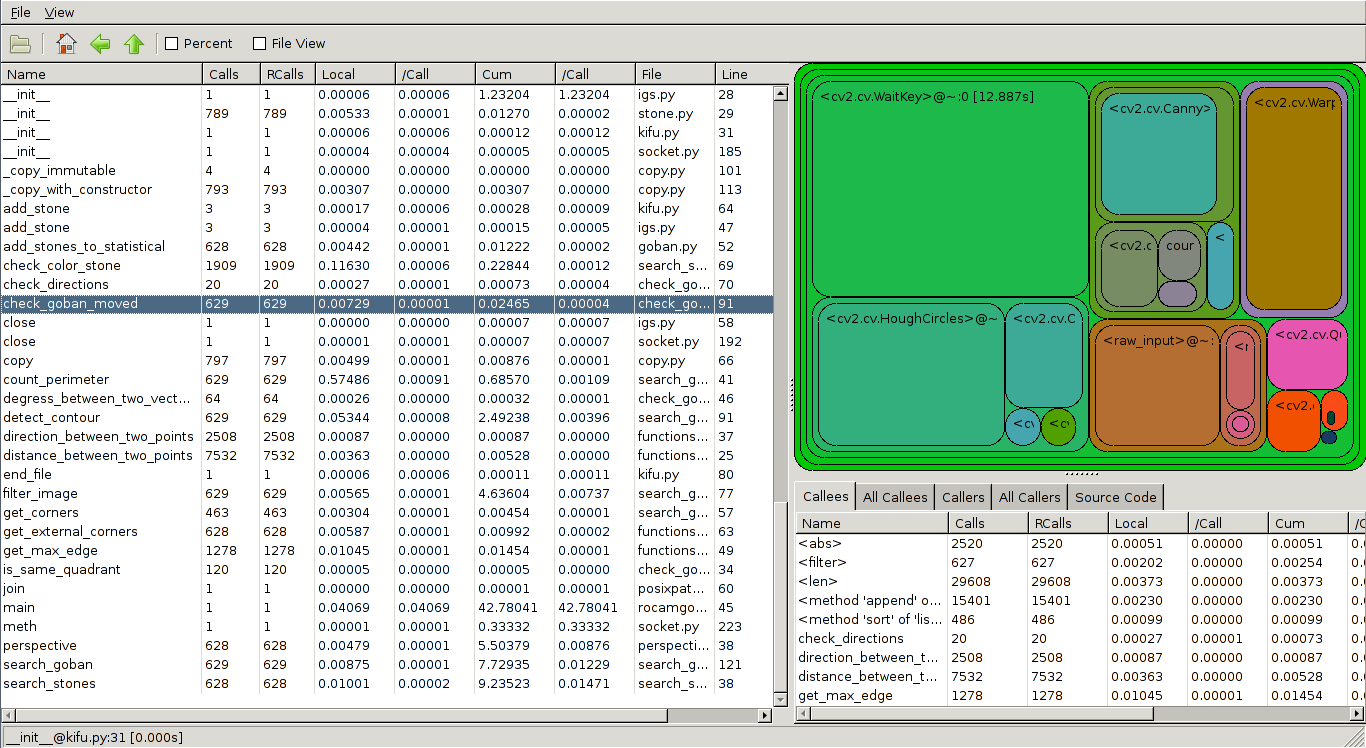
\includegraphics[scale=0.33]{runsnake.png}

\subsubsection{Conclusiones}

Para hacer profiling en este proyecto hemos utilizado los tres profilers
mencionados anteriormente, Profiler y cProfiler funcionan exactamente igual, con
la diferencia de que uno está escrito en C y otro en python, por lo cual,
intentamos utilizar en un principio cProfiler, que funciona con mayor rapidez, y
si este no podemos importarlo, utilizamos Profiler, que está escrito en
python. Esto lo utilizamos ejecutando nuestro proyecto, con lo cual tenemos que
ir interactuando con él para qué vaya haciendo las llamadas necesarias y
comprobar que funciones tardan más y donde pueden existir cuellos de botella. 
El hotshot lo utilizamos por que al realizar los test, la herramienta de
nosetest tiene la funcionalidad de comprobar el rendimiento del código
utilizando esta herramienta de profiling. La salida que genera no podemos leerla
con runsnake, para ello, tenemos que transformar esa salida utilizando
$hotshot2stats.py$


\subsection{Editores de texto: Geany, Gedit y Vim}

\subsubsection{Geany} 

Es un editor de texto ligero basado en Scintilla con características básicas de
entorno de desarrollo integrado (IDE). Está disponible para distintos sistemas
operativos, como GNU/Linux, Mac OS X, BSD, Solaris y Microsoft Windows.  Es
distribuido como software libre bajo la Licencia Pública General de GNU.

\parskip 2ex
Nostros empezamos a utilizar este editor ya que nos fácilitaba el autocompletado
y era bastante liviano, tenía coloreado de sintaxis y permitía la programación
con el lenguaje usado por nosotros, Python. 

\subsubsection{Gedit}

es un editor de textos compatible con UTF-8 para GNU/Linux, Mac OS X y Microsoft
Windows. Diseñado como un editor de textos de propósito general, gedit enfatiza
la simplicidad y fácilidad de uso. Incluye herramientas para la edición de
código fuente y textos estructurados, como lenguajes de marcado. Distribuido
bajo las condiciones de la licencia GPL, gedit es software libre. 

\parskip 2ex
Nosotros cambiamos a este editor por que aún era más simple y liviano que Geany,
y aunque no nos daba un buen autocompletado, tenía todo lo que queríamos,
coloreado de sintáxis, fácilidad de uso, y también hay que tener en cuenta que
es el editor por defecto del entorno de escritorio GNOME, el cual hemos
utilizado bastante. 

\parskip 2ex

\subsubsection{Vim}

Es un editor hecho por programadores para programadores. Para fácilitar la
programación, Vim dispone de un modo 'editar, compilar, corregir'.  De la misma
forma que los entornos de desarrollo integrados, puede editar el código fuente
además llamar a un compilador externo, e interpretar sus resultados. Si hay
errores de compilación, éstos se muestran en una ventana. Los mensajes de error
dirigen al usuario a la zona en la que se han encontrado para poder así
corregirlos. Entonces vuelve a empezar el ciclo "editar, compilar, corregir" y,
si es necesario, corregir nuevos errores. El trabajo del programador también se
ve fácilitado por el resaltado de sintaxis y la funcionalidad de plegado de
código.

\parskip 2ex 
Empezamos a utilizar este editor ya que está preparado para
programadores, y su filosofía se basa es hacerlo todo con el mínimo número de
pulsaciones de teclado, lo cual, cuando nos acostumbremos a utilizarlo,
conseguiremos una gran mejora de productividad. También decir que Vim es el
programa que actualmente más plugins tiene, y es altamente configurable, para
adecuarse al perfil de cada programador, cosa que nos ha gustado muchísimo. 


\subsection{Servidores de Go: IGS y KGS}

\subsubsection{El servidor IGS}

Nos ofrece un gran lugar para jugar, ver, estudiar y disfrutar del juego de Go
en Internet. Podemos encontrar cientos de jugadores de dintintas partes del
mundo y diferentes nivelesde juego, desde principiantes hasta profesionales. 

\parskip 2ex
Además este servidor ofrece un protocolo de comunicaciones abierto y muy bien
documentado, el cual hemos utilizado para subir la partida mientras se va
jugando. 

\subsubsection{KGS Go Server}

Llamado comunmente KGS, es un servidor de Go popular al cual podemos acceder
desde http://www.gokgs.com/. Normalmente hay más de 1500 personas conectadas en
cualquier momento, por lo que es uno de los servidores más grandes en el mundo.
Muchas de las partidas de perfil alto de los torneos se retransmiten en KGS. KGS
abrió por primera vez bajo el nombre Igoweb en abril de 2000.  Apenas un mes
después, el autor hizo un acuerdo con Kiseido y fue rebautizado con el Kiseido
Go Server. Su nombre se cambió a KGS Go Server en 2006. William M. Shubert es el
desarrollador de KGS. El cliente conocido como CGoban3 ha sido escrito en
Inglés, y ha sido traducido a muchos idiomas diferentes, como japonés, francés,
italiano, alemán, chino y español entre otros. 

\parskip 2ex
Nosotros también hemos intentado subir la partida a este servidor, pero el
protocolo de comunicación que se usa no es software libre, por lo tanto no
tenemos acceso a él para subir una partida fácilmente, ya que no hemos
encontrado tampoco mucha comunicación. En estos momentos estamos intercambiando
correos con el desarrollador de KGS y algunos administradores para ver si
podemos hacer algo y que se permitan subir partidas a este servidor tan
conocido. 


\subsection{Sistemas Operativos: Debian y Linux Mint}

\subsubsection{Debian}

Es un sistema operativo libre, desarrollado por más de mil voluntarios alrededor
del mundo, que colaboran a través de Internet.  La dedicación de Debian al
software libre, su base de voluntarios, su naturaleza no comercial y su modelo
de desarrollo abierto la distingue de otras distribuciones del sistema operativo
GNU. Todos estos aspectos y más se recogen en el llamado Contrato Social de
Debian.  Nació en el año 1993, de la mano del proyecto Debian, con la idea de
crear un sistema GNU usando Linux como núcleo ya que el proyecto Debian,
organización responsable de su mantenimiento en la actualidad, también
desarrolla sistemas GNU basados en otros núcleos (Debian GNU/Hurd, Debian
GNU/NetBSD y Debian GNU/kFreeBSD).  Uno de sus principales objetivos es separar
en sus versiones el software libre del software no libre. El modelo de
desarrollo es independiente a empresas, creado por los propios usuarios, sin
depender de ninguna manera de necesidades comerciales. Debian no vende
directamente su software, lo pone a disposición de cualquiera en Internet,
aunque sí permite a personas o empresas distribuir comercialmente este software
mientras se respete su licencia.  Debian Linux puede instalarse utilizando
distintos mecanismos de instalación, como DVD, CD, Blu-Ray, memorias USB y
diskettes, e incluso directamente desde la red.

\subsubsection{Linux Mint}

Es una distribución del sistema operativo GNU/Linux, basado en la distribución
Ubuntu (que a su vez está basada en Debian). A partir del 7 de septiembre de
2010 también está disponible una edición basada en Debian.  Linux Mint mantiene
un inventario actualizado, un sistema operativo estable para el usuario medio,
con un fuerte énfasis en la usabilidad y fácilidad de instalación. Es reconocido
por ser fácil de usar, especialmente para los usuarios sin experiencia previa en
Linux.  Linux Mint se compone de muchos paquetes de software, los cuales se
distribuyen la mayor parte bajo una licencia de software libre. La principal
licencia utilizada es la GNU General Public License (GNU GPL) que, junto con la
GNU Lesser General Public License (GNU LGPL), declara explícitamente que los
usuarios tienen libertad para ejecutar, copiar, distribuir, estudiar, cambiar,
desarrollar y mejorar el software. Linux Mint es financiada por su comunidad de
usuarios. Los usuarios individuales y empresas que utilizan el sistema operativo
pueden actuar como donantes, patrocinadores y socios de la distribución. El
apoyo financiero de la comunidad y la publicidad en el sitio web ayuda a
mantener Linux Mint libre y abierta.

\subsubsection{Conclusiones}

Como puede observarse, hemos intentado utilizar todas las herramientas libres
que hemos visto necesarias, incluyendo, como no, el sistema operativo. Como cada uno
tenemos nuestros gustos, cada uno de nosotros hemos utilizados el sitema
operativo que más se adecuaba a nuestros gustos. 


\subsection{Entornos de escritorio: Awesome y Cinnamon}

\subsubsection{Awesome}

Es un gestor de ventanas para X Window System desarrollado en C y lenguaje de
programación Lua. Este último también se utiliza para configurar y ampliar el
gestor de ventanas. Al igual que muchos gestores de ventanas del tipo tiling
window manager (tipo mosaico), hace lo posible para qué el usuario pueda manejar
productivamente las ventanas sin el uso del ratón.  El programa se incorpora en
los repositorios de Debian GNU/Linux desde la versión lenny en su versión 2. La
nueva versión, 3.4.2 For The Restless, se encuentra en los repositorios de
Ubuntu y en la versión estable de Debian.

\subsubsection{Cinnamon}

Es una bifurcación de GNOME Shell, desarrollado inicialmente por Linux Mint.
Intenta proveer un entorno de escritorio más tradicional basado en la metáfora
de escritorio, como GNOME 2. Cinnamon usa Muffin, una bifurcación del gestor de
ventanas de GNOME 3 Mutter, como su gestor de ventanas desde la versión 1.2.

\subsubsection{Conclusiones}

Al igual que con el sistema operativo ha ocurrido con el entorno de escritorio,
gracias a que en la comunidad del Software Libre se ofrecen inifinidad de
posibilidades de entornos, cada uno hemos utilizado el que más nos gustaba.


\chapter{Implementación}

\section{Estrutura interna del proyecto}

La estructura de este proyecto la hemos dividido por funcionalidades, para
intentar que el código sea lo más legible, entendible y reutlizable posible. Las
funcionalidades en las que hemos dividido el proyecto son la siguientes:
\begin{itemize} 
    \item Selección de cámara o video para la captura de una partida.
    \item Detección de cámaras. 
    \item Detección de tablero.
    \item Comprobación del movimiento del tablero.
    \item Idealización del tablero.
    \item Detección de piedras.
    \item Procesamiento de piedras. 
    \item Comunicación con el servidor. Transmisión de partida por Internet.
\end{itemize}

La realización de este proyecto a supuesto muchísimos cambios en las
implementaciones, ya que hemos tenido que desechar muchas de ellas por motivos
diferentes que nos hemos ido encontrando. Hemos decidido ir explicando la
evolución y aprendizaje de cada parte de software del proyecto, añadiendo
despues la api correspondiente a esa parte. A continuación adjuntamos la api del
main.

%
% API Documentation for API Documentation
% Module src.rocamgo
%
% Generated by epydoc 3.0.1
% [Wed Sep 12 02:49:43 2012]
%

%%%%%%%%%%%%%%%%%%%%%%%%%%%%%%%%%%%%%%%%%%%%%%%%%%%%%%%%%%%%%%%%%%%%%%%%%%%
%%                          Module Description                           %%
%%%%%%%%%%%%%%%%%%%%%%%%%%%%%%%%%%%%%%%%%%%%%%%%%%%%%%%%%%%%%%%%%%%%%%%%%%%

    \index{src \textit{(package)}!src.rocamgo \textit{(module)}|(}
\section{Module src.rocamgo}

    \label{src:rocamgo}

%%%%%%%%%%%%%%%%%%%%%%%%%%%%%%%%%%%%%%%%%%%%%%%%%%%%%%%%%%%%%%%%%%%%%%%%%%%
%%                               Functions                               %%
%%%%%%%%%%%%%%%%%%%%%%%%%%%%%%%%%%%%%%%%%%%%%%%%%%%%%%%%%%%%%%%%%%%%%%%%%%%

  \subsection{Functions}

    \label{src:rocamgo:main}
    \index{src \textit{(package)}!src.rocamgo \textit{(module)}!src.rocamgo.main \textit{(function)}}

    \vspace{0.5ex}

\hspace{.8\funcindent}\begin{boxedminipage}{\funcwidth}

    \raggedright \textbf{main}()

\setlength{\parskip}{2ex}
\setlength{\parskip}{1ex}
    \end{boxedminipage}


%%%%%%%%%%%%%%%%%%%%%%%%%%%%%%%%%%%%%%%%%%%%%%%%%%%%%%%%%%%%%%%%%%%%%%%%%%%
%%                               Variables                               %%
%%%%%%%%%%%%%%%%%%%%%%%%%%%%%%%%%%%%%%%%%%%%%%%%%%%%%%%%%%%%%%%%%%%%%%%%%%%

  \subsection{Variables}

    \vspace{-1cm}
\hspace{\varindent}\begin{longtable}{|p{\varnamewidth}|p{\vardescrwidth}|l}
\cline{1-2}
\cline{1-2} \centering \textbf{Name} & \centering \textbf{Description}& \\
\cline{1-2}
\endhead\cline{1-2}\multicolumn{3}{r}{\small\textit{continued on next page}}\\\endfoot\cline{1-2}
\endlastfoot\raggedright \_\-\_\-p\-a\-c\-k\-a\-g\-e\-\_\-\_\- & \raggedright \textbf{Value:} 
{\tt \texttt{'}\texttt{src}\texttt{'}}&\\
\cline{1-2}
\raggedright c\-a\-m\- & \raggedright Objeto Cameras

            {\it (type=Cameras)}&\\
\cline{1-2}
\raggedright c\-a\-m\-e\-r\-a\- & \raggedright cámara que estamos usando

            {\it (type=Camera)}&\\
\cline{1-2}
\raggedright c\-a\-m\-s\-\_\-f\-o\-u\-n\-d\- & \raggedright número de cámaras encontradas en el ordenador

            {\it (type=int)}&\\
\cline{1-2}
\raggedright c\-i\-r\-c\-l\-e\-s\- & \raggedright circulos encontrado en la imagen

            {\it (type=CvMat)}&\\
\cline{1-2}
\raggedright c\-o\-l\-o\-r\- & \raggedright color de la piedra

            {\it (type=int)}&\\
\cline{1-2}
\raggedright c\-u\-r\-r\-e\-n\-t\-\_\-c\-o\-r\-n\-e\-r\-s\- & \raggedright esquinas actuales del tablero encontradas

            {\it (type=list)}&\\
\cline{1-2}
\raggedright f\-a\-l\-s\-e\-\_\-s\-t\-o\-n\-e\-s\- & \raggedright contador para piedras falsas, no son negras o blancas

            {\it (type=int)}&\\
\cline{1-2}
\raggedright g\-o\-b\-a\-n\- & \raggedright Objeto tablero

            {\it (type=Goban)}&\\
\cline{1-2}
\raggedright g\-o\-o\-d\-\_\-c\-o\-r\-n\-e\-r\-s\- & \raggedright últimas esquinas buenas encontradas

            {\it (type=list)}&\\
\cline{1-2}
\raggedright i\-d\-e\-a\-l\-\_\-i\-m\-g\- & \raggedright tablero en formato ideal

            {\it (type=IplImage)}&\\
\cline{1-2}
\raggedright i\-m\-g\- & \raggedright imagen actual sacada de la cámara o video

            {\it (type=IplImage)}&\\
\cline{1-2}
\raggedright k\-e\-y\- & \raggedright tecla pulsada

            {\it (type=int)}&\\
\cline{1-2}
\raggedright p\-r\-e\-v\-\_\-c\-o\-r\-n\-e\-r\-s\- & \raggedright esquinas del tablero anteriores encontradas

            {\it (type=list)}&\\
\cline{1-2}
\raggedright p\-t\- & \raggedright centro de la piedra

            {\it (type=tuple)}&\\
\cline{1-2}
\raggedright r\-a\-d\-i\-o\-u\-s\- & \raggedright radio de la piedra

            {\it (type=float)}&\\
\cline{1-2}
\raggedright s\-t\-o\-n\-e\-s\- & \raggedright piedras detectadas como negras o blancas

            {\it (type=list)}&\\
\cline{1-2}
\end{longtable}

    \index{src \textit{(package)}!src.rocamgo \textit{(module)}|)}


\section{Selección de cámara o video para la captura de una partida} 

Esta funcionalidad nos permite seleccionar si queremos utilizar una cámara o un
video grabado anteriormente para comenzar la captura y subida de la partida a
Internet.

La opción de cargar un video nos ha servido mayormente a los desarrolladores
para testear si todo funcionaba correctamente, hemos ido cargando videos previamente
grabados con situaciones reales que podemos encontrarnos en cualquier tipo de
partidas.


\section{Detección de la cámara} 

Funcionalidad que nos busca las cámaras que se encuentren enchufadas al PC y nos
las devuelve para qué seleccionemos la que queramos utilizar. Si no existen
cámaras conectadas al PC, tendremos que usar la funcionalidad de utilizar un
video como captura para ver el funcionamiento de este proyecto.  

\subsection{1ª Implementación: detección de cámaras solo en Linux}

Nuestra primera detección de cámaras solo estaba preparada para funcionar en
Linux, ya que utilizábamos una manera que solo funcionaba en Linux, y la cual,
si enchufabas y desenchufabas alguna cámara anteriormente, daba fallos, ya que
capturábamos las cámaras utilizando el dispositivo de video que se encontraban
en las direcciones /dev/videoX, siendo X el número de la cámara. Esta fué una
solución rápida y fácil a la hora de seleccionar cámaras, y fue posible gracias
al conocimiento sobre como funcionan los dispositivos en Linux y donde se
encuentran ubicados. 

Respecto a la selección de la cámara, no hemos utilizado ninguna interfaz
visual, las ventanas donde seleccionamos las cámara las creamos con OpenCv,
aunque pensamos que en un futuro podríamos utilizar alguna interfaz. 

\subsection{2ª Implmentación: detección de cámaras utilizando OpenCv}

Esta implementación funciona bastante bien, ya que no solo funciona en Linux, si
no que también funciona en Windows y debería de funcionar en MAC. No hemos
podido hacer la comprobación en MAC ya que no disponemos de ningún dispositivo
con este sistema operativo. Tenemos que destacar que esta forma es una forma
mejorada de detectar las cámaras, ya que no hay problemas si hemos enchufado y
desenchufado cámaras anteriormente.

En esta segunda implementación no hemos cambiado la forma de seleccionar las
cámaras y seguimos utilizando OpenCv para la selección. 

%
% API Documentation for API Documentation
% Module src.camera
%
% Generated by epydoc 3.0.1
% [Sun Sep  9 21:09:35 2012]
%

%%%%%%%%%%%%%%%%%%%%%%%%%%%%%%%%%%%%%%%%%%%%%%%%%%%%%%%%%%%%%%%%%%%%%%%%%%%
%%                          Module Description                           %%
%%%%%%%%%%%%%%%%%%%%%%%%%%%%%%%%%%%%%%%%%%%%%%%%%%%%%%%%%%%%%%%%%%%%%%%%%%%

    \index{src \textit{(package)}!src.camera \textit{(module)}|(}
\section{Module src.camera}

    \label{src:camera}

%%%%%%%%%%%%%%%%%%%%%%%%%%%%%%%%%%%%%%%%%%%%%%%%%%%%%%%%%%%%%%%%%%%%%%%%%%%
%%                               Variables                               %%
%%%%%%%%%%%%%%%%%%%%%%%%%%%%%%%%%%%%%%%%%%%%%%%%%%%%%%%%%%%%%%%%%%%%%%%%%%%

  \subsection{Variables}

    \vspace{-1cm}
\hspace{\varindent}\begin{longtable}{|p{\varnamewidth}|p{\vardescrwidth}|l}
\cline{1-2}
\cline{1-2} \centering \textbf{Name} & \centering \textbf{Description}& \\
\cline{1-2}
\endhead\cline{1-2}\multicolumn{3}{r}{\small\textit{continued on next page}}\\\endfoot\cline{1-2}
\endlastfoot\raggedright \_\-\_\-p\-a\-c\-k\-a\-g\-e\-\_\-\_\- & \raggedright \textbf{Value:} 
{\tt \texttt{'}\texttt{src}\texttt{'}}&\\
\cline{1-2}
\end{longtable}


%%%%%%%%%%%%%%%%%%%%%%%%%%%%%%%%%%%%%%%%%%%%%%%%%%%%%%%%%%%%%%%%%%%%%%%%%%%
%%                           Class Description                           %%
%%%%%%%%%%%%%%%%%%%%%%%%%%%%%%%%%%%%%%%%%%%%%%%%%%%%%%%%%%%%%%%%%%%%%%%%%%%

    \index{src \textit{(package)}!src.camera \textit{(module)}!src.camera.Camera \textit{(class)}|(}
\subsection{Class Camera}

    \label{src:camera:Camera}
Clase para inicializar la cámara.


%%%%%%%%%%%%%%%%%%%%%%%%%%%%%%%%%%%%%%%%%%%%%%%%%%%%%%%%%%%%%%%%%%%%%%%%%%%
%%                                Methods                                %%
%%%%%%%%%%%%%%%%%%%%%%%%%%%%%%%%%%%%%%%%%%%%%%%%%%%%%%%%%%%%%%%%%%%%%%%%%%%

  \subsubsection{Methods}

    \label{src:camera:Camera:__init__}
    \index{src \textit{(package)}!src.camera \textit{(module)}!src.camera.Camera \textit{(class)}!src.camera.Camera.\_\_init\_\_ \textit{(method)}}

    \vspace{0.5ex}

\hspace{.8\funcindent}\begin{boxedminipage}{\funcwidth}

    \raggedright \textbf{\_\_init\_\_}(\textit{self})

\setlength{\parskip}{2ex}
\setlength{\parskip}{1ex}
    \end{boxedminipage}

    \label{src:camera:Camera:open_camera}
    \index{src \textit{(package)}!src.camera \textit{(module)}!src.camera.Camera \textit{(class)}!src.camera.Camera.open\_camera \textit{(method)}}

    \vspace{0.5ex}

\hspace{.8\funcindent}\begin{boxedminipage}{\funcwidth}

    \raggedright \textbf{open\_camera}(\textit{self}, \textit{index})

    \vspace{-1.5ex}

    \rule{\textwidth}{0.5\fboxrule}
\setlength{\parskip}{2ex}
    Abrir cámara con opencv. :param index: índice de la cámara. :type 
    index: int.

\setlength{\parskip}{1ex}
    \end{boxedminipage}

    \label{src:camera:Camera:get_frame}
    \index{src \textit{(package)}!src.camera \textit{(module)}!src.camera.Camera \textit{(class)}!src.camera.Camera.get\_frame \textit{(method)}}

    \vspace{0.5ex}

\hspace{.8\funcindent}\begin{boxedminipage}{\funcwidth}

    \raggedright \textbf{get\_frame}(\textit{self})

    \vspace{-1.5ex}

    \rule{\textwidth}{0.5\fboxrule}
\setlength{\parskip}{2ex}
    Obtener una imagen desde la cámara.

\setlength{\parskip}{1ex}
    \end{boxedminipage}

    \label{src:camera:Camera:is_open}
    \index{src \textit{(package)}!src.camera \textit{(module)}!src.camera.Camera \textit{(class)}!src.camera.Camera.is\_open \textit{(method)}}

    \vspace{0.5ex}

\hspace{.8\funcindent}\begin{boxedminipage}{\funcwidth}

    \raggedright \textbf{is\_open}(\textit{self})

    \vspace{-1.5ex}

    \rule{\textwidth}{0.5\fboxrule}
\setlength{\parskip}{2ex}
    Comprueba si la cámara está abierta.

\setlength{\parskip}{1ex}
    \end{boxedminipage}

    \label{src:camera:Camera:close_camera}
    \index{src \textit{(package)}!src.camera \textit{(module)}!src.camera.Camera \textit{(class)}!src.camera.Camera.close\_camera \textit{(method)}}

    \vspace{0.5ex}

\hspace{.8\funcindent}\begin{boxedminipage}{\funcwidth}

    \raggedright \textbf{close\_camera}(\textit{self})

    \vspace{-1.5ex}

    \rule{\textwidth}{0.5\fboxrule}
\setlength{\parskip}{2ex}
    Cierra la cámara.

\setlength{\parskip}{1ex}
    \end{boxedminipage}

    \index{src \textit{(package)}!src.camera \textit{(module)}!src.camera.Camera \textit{(class)}|)}
    \index{src \textit{(package)}!src.camera \textit{(module)}|)}

%
% API Documentation for API Documentation
% Módulo src.cameras
%
% Generated by epydoc 3.0.1
% [Wed Sep 12 04:59:27 2012]
%

%%%%%%%%%%%%%%%%%%%%%%%%%%%%%%%%%%%%%%%%%%%%%%%%%%%%%%%%%%%%%%%%%%%%%%%%%%%
%%                          Módulo Description                           %%
%%%%%%%%%%%%%%%%%%%%%%%%%%%%%%%%%%%%%%%%%%%%%%%%%%%%%%%%%%%%%%%%%%%%%%%%%%%

    \index{src \textit{(package)}!src.cameras \textit{(module)}|(}
\section{Módulo src.cameras}

    \label{src:cameras}

%%%%%%%%%%%%%%%%%%%%%%%%%%%%%%%%%%%%%%%%%%%%%%%%%%%%%%%%%%%%%%%%%%%%%%%%%%%
%%                               Variables                               %%
%%%%%%%%%%%%%%%%%%%%%%%%%%%%%%%%%%%%%%%%%%%%%%%%%%%%%%%%%%%%%%%%%%%%%%%%%%%

  \subsection{Variables}

    \vspace{-1cm}
\hspace{\varindent}\begin{longtable}{|p{\varnamewidth}|p{\vardescrwidth}|l}
\cline{1-2}
\cline{1-2} \centering \textbf{Nombre} & \centering \textbf{Description}& \\
\cline{1-2}
\endhead\cline{1-2}\multicolumn{3}{r}{\small\textit{continua en la página siguiente}}\\\endfoot\cline{1-2}
\endlastfoot\raggedright \_\-\_\-p\-a\-c\-k\-a\-g\-e\-\_\-\_\- & \raggedright \textbf{Valor:} 
{\tt \texttt{'}\texttt{src}\texttt{'}}&\\
\cline{1-2}
\raggedright c\-a\-m\-e\-r\-a\- & \raggedright cámara seleccionada

            {\it (tipo=Capture)}&\\
\cline{1-2}
\raggedright c\-a\-m\-e\-r\-a\-s\- & \raggedright lista de cámaras

            {\it (tipo=list)}&\\
\cline{1-2}
\end{longtable}


%%%%%%%%%%%%%%%%%%%%%%%%%%%%%%%%%%%%%%%%%%%%%%%%%%%%%%%%%%%%%%%%%%%%%%%%%%%
%%                           Clase Description                           %%
%%%%%%%%%%%%%%%%%%%%%%%%%%%%%%%%%%%%%%%%%%%%%%%%%%%%%%%%%%%%%%%%%%%%%%%%%%%

    \index{src \textit{(package)}!src.cameras \textit{(module)}!src.cameras.Cameras \textit{(class)}|(}
\subsection{Clase Cameras}

    \label{src:cameras:Cameras}

Clase para abrir las cámaras disponibles en el ordenador.

%%%%%%%%%%%%%%%%%%%%%%%%%%%%%%%%%%%%%%%%%%%%%%%%%%%%%%%%%%%%%%%%%%%%%%%%%%%
%%                                Métodos                                %%
%%%%%%%%%%%%%%%%%%%%%%%%%%%%%%%%%%%%%%%%%%%%%%%%%%%%%%%%%%%%%%%%%%%%%%%%%%%

  \subsubsection{Métodos}

    \label{src:cameras:Cameras:__init__}
    \index{src \textit{(package)}!src.cameras \textit{(module)}!src.cameras.Cameras \textit{(class)}!src.cameras.Cameras.\_\_init\_\_ \textit{(method)}}

    \vspace{0.5ex}

\hspace{.8\funcindent}\begin{boxedminipage}{\funcwidth}

    \raggedright \textbf{\_\_init\_\_}(\textit{self})

\setlength{\parskip}{2ex}
\setlength{\parskip}{1ex}
    \end{boxedminipage}

    \label{src:cameras:Cameras:on_mouse}
    \index{src \textit{(package)}!src.cameras \textit{(module)}!src.cameras.Cameras \textit{(class)}!src.cameras.Cameras.on\_mouse \textit{(method)}}

    \vspace{0.5ex}

\hspace{.8\funcindent}\begin{boxedminipage}{\funcwidth}

    \raggedright \textbf{on\_mouse}(\textit{self}, \textit{event}, \textit{x}, \textit{y}, \textit{flags}, \textit{camera})

    \vspace{-1.5ex}

    \rule{\textwidth}{0.5\fboxrule}
\setlength{\parskip}{2ex}
Capturador de eventos de click de ratón.

\setlength{\parskip}{1ex}
      \textbf{Parametros}
      \vspace{-1ex}

      \begin{quote}
        \begin{Ventry}{xxxxxx}

          \item[event]


Evento capturado.
            {\it (tipo=int)}

          \item[x]


posición x del ratón.
            {\it (tipo=int)}

          \item[y]


posición y del ratón.
            {\it (tipo=int)}

          \item[camera]


objeto Camera.
            {\it (tipo=Camera)}

        \end{Ventry}

      \end{quote}

    \end{boxedminipage}

    \label{src:cameras:Cameras:check_cameras}
    \index{src \textit{(package)}!src.cameras \textit{(module)}!src.cameras.Cameras \textit{(class)}!src.cameras.Cameras.check\_cameras \textit{(method)}}

    \vspace{0.5ex}

\hspace{.8\funcindent}\begin{boxedminipage}{\funcwidth}

    \raggedright \textbf{check\_cameras}(\textit{self}, \textit{num}={\tt 99})

    \vspace{-1.5ex}

    \rule{\textwidth}{0.5\fboxrule}
\setlength{\parskip}{2ex}
Comprueba las cámaras disponibles.

\setlength{\parskip}{1ex}
      \textbf{Parametros}
      \vspace{-1ex}

      \begin{quote}
        \begin{Ventry}{xxx}

          \item[num]


máximo número de cámaras a comprobar
          \item[num]


99 por defecto, ya que en Linux es lo permitido
          \item[num]


int
        \end{Ventry}

      \end{quote}

      \textbf{Return Valor}
    \vspace{-1ex}

      \begin{quote}

lista de cámaras disponibles
      {\it (tipo=list of Camera)}

      \end{quote}

    \end{boxedminipage}

    \label{src:cameras:Cameras:show_and_select_camera}
    \index{src \textit{(package)}!src.cameras \textit{(module)}!src.cameras.Cameras \textit{(class)}!src.cameras.Cameras.show\_and\_select\_camera \textit{(method)}}

    \vspace{0.5ex}

\hspace{.8\funcindent}\begin{boxedminipage}{\funcwidth}

    \raggedright \textbf{show\_and\_select\_camera}(\textit{self})

    \vspace{-1.5ex}

    \rule{\textwidth}{0.5\fboxrule}
\setlength{\parskip}{2ex}
Muestra las cámaras disponibles en ventanas y da la opción de seleccionar una de ellas pulsando doble click.

\setlength{\parskip}{1ex}
      \textbf{Return Valor}
    \vspace{-1ex}

      \begin{quote}

cámara seleccionada
      {\it (tipo=Camera)}

      \end{quote}

    \end{boxedminipage}

    \index{src \textit{(package)}!src.cameras \textit{(module)}!src.cameras.Cameras \textit{(class)}|)}
    \index{src \textit{(package)}!src.cameras \textit{(module)}|)}


\section{Detección del tablero} 

Funcionalidad para la detección del tablero, ya sea de las intersecciones o de
las esquinas, para luego poder ubicar la posición de las piedras de alguna
manera. Esta funcionalidad es de una de las que nos ha costado más que funcione
más o menos bien la mayoría de las veces, ya que con la última implementación
seguimos encontrando algunos pequeños errores en la detección de tablero
diferentes. 

\subsection{1ª Implementación: detección mediante líneas}

En este intento de implementación intentamos buscar las líneas del tablero 
mediante el tratamiento de imágenes y la función HoughLines de OpenCv, para 
luego buscar las intersecciones del tablero y así tener el tablero detectado. 
Pensamos que el tratamiento de esas líneas sería sencillo de procesar, pero al
existir tantas líneas y tener que buscar tantas intersecciones, se convertía en
un procesamiento tan inmeso que no fuimos capaces de abordar, y por tanto,
descartamos al ver que con esta forma, tardaríamos muchísimo en encontrar la
posición del tablero.

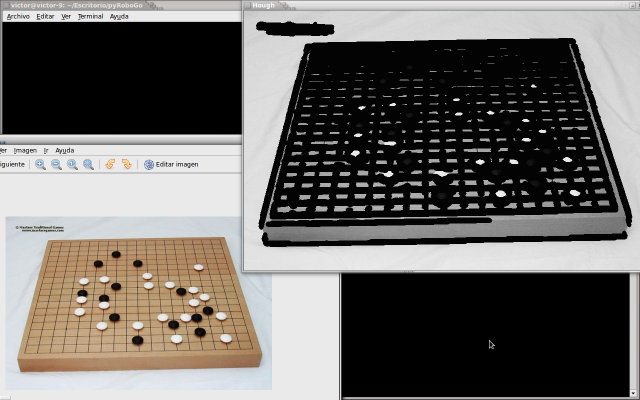
\includegraphics[scale=0.6]{detect-lineas.png}

Otro de los problemas era que el tablero estaría casi siempre con un poco de
perspectiva, y entonces no sabríamos que líneas escoger, ya que el tablero, al
ser de madera contiene muchas betas y podría detectar bastantes líneas que no
serían las buscadas. 
Más adelante nos dimos cuenta de que existe otro problema con esta
implementación, y es que cuando existan piedras encima del tablero, estas líneas
serán tapadas, evitando así poder detectar el tablero más adelante.
 

\subsection{2ª Implementación: detección mediante intersecciones}

Despues de entender que la forma anterior de buscar el tablero no era efectiva,
decidimos ponernos a trabajar en otra idea. Esta vez decidimos hacerlo, atacando
a las intersecciones, usando templates. Esta forma consiste en buscar en la
imagen que recibimos de la cámara, el template de una intersección (imagen
que contine solo la intersección). Con esto conseguíamos detectar casi a la
perfección casi todas las intersecciones, y las que no, podíamos sacarlas
mediante una malla y unos cuantos de cálculos.

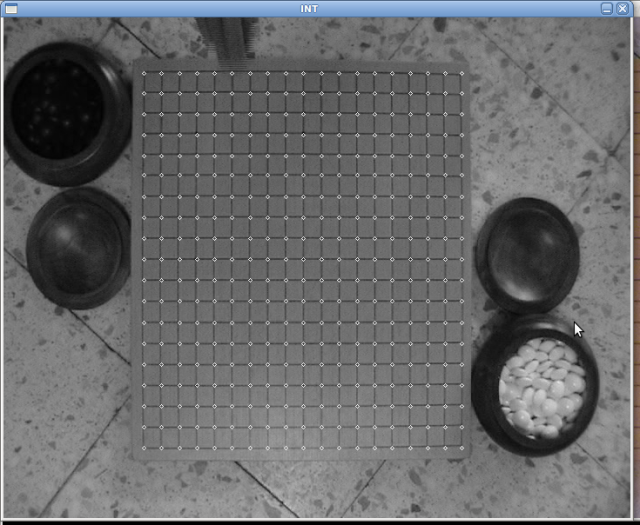
\includegraphics[scale=0.6]{detec-intersecciones.png}

El problema que nos encontramos con esta implementación, era el coste de
ejecución que conllevaba todo este proceso y, a parte, también nos toparíamos
con el problema que hemos mencionado anteriormente de la perspectiva, ya que a
la más mínima perspectiva, el template ideal no nos serviría, y el coste para
detectar esto sería aun mayor. 
También nos encontramos con otro de los problemas que vimos en la anterior
implementación, el de que las piedras taparían en el transcurso de la partida
estas intersecciones, con lo cual no podríamos encontrarlas utilizando
templates.

\subsection{3ª Implementación: Haartraining, aprendizaje}

Tras dos intentos fallidos, comenzamos a estudiar la siguiente idea, sacada de
distintos programas de cámaras de fotos, los cuales detectan y recuadran la
cara. Esta forma de hacerlo se llama HaarTraining, y consiste en enseñarle al
ordenador a buscar un tablero, introduciendo en un programa de aprendizaje
imágenes donde estén los tableros, indicandole la posición. En ese proceso de
aprendizaje también hay que enseñarle fotos que no contengan el tablero.
Después de estudiarlo, nos dimos cuenta de varias cosas que hicieron que no
continuásemos por este camino. La primera de ellas es el tiempo dedicado a la
realización de las fotos y posterior análisis manual, para indicar el lugar del
tablero. La segunda el tiempo de ejecución del aprendizaje, suele llevar unas
dos semanas, en un ordenador potente. Y por último, la tercea y más importante,
es que despues de las dos primeras, nadie te aseguraba con una minima certeza 
que esta posibilidad fuese a funcionar.

En la siguiente imagen podemos ver un claro ejemplo que usan las cámaras de foto
con este tipo de implementación.

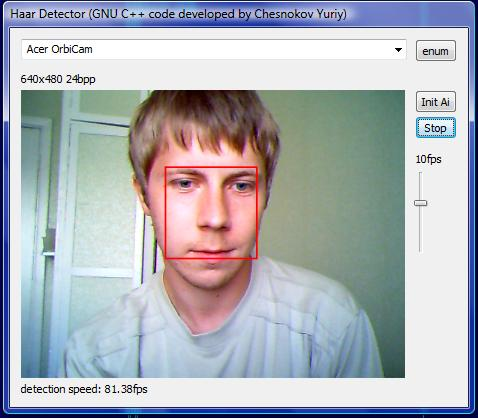
\includegraphics[scale=1]{haartraining.jpg} 

Estuvimos bastante tiempo investigando y probamos con 40-50 imágenes, en vez de
con 3000 como mínimo, que es lo que piden, y como esperábamos, fue un fracaso,
no encontraba tablero ninguno con tan pocas imágenes de aprendizaje. 


\subsection{4ª Implementación: detección mediante contornos}

Finalmente, y tras tres intentos fallidos, decidimos hacerlo buscando contornos.
Gracias a una función de OpenCv conseguimos encontrar la forma que menos fallos
nos ha dado, cumple con los requisitos y soluciona casi todos los problemas.
Esta función devuelve contornos, por ello uno de los requisitos que debemos
pedir para la correcta ejecución de este programa es que el fondo donde se
coloque el tablero, sea lo más liso posible, cosa que podemos conseguir con
fácilidad utilizando un mantel o hule, aunque no es totalmente necesario, pero
fácilita y ayuda al mejor funcionamiento del programa. Debido a la gran cantidad
de test que ha pasado correctamente esta implementación y dado que los test que
han fallado son debido a la mala calidad de las imágenes (sobre todo a causa de
la luminosidad de las imágenes), hemos considerado que es la correcta. Además,
perdemos el problema de la perspectiva, pues lo que detectamos es el contorno.

Cabe destacar de esta implementación, que la búsqueda de contornos nos encuentra
muchas veces el contorno de la imagen completa, el cual tendremos que desechar
comprobando que el contorno es demasiado grande para ser del tablero. También
nos ocurre lo mismo con cualquier contorno más pequeño que encontremos. Por
último, y como lo que estamos buscando es una tablero, el cual es rectangular,
tenemos que hacer aproximaciones de estos contornos y descartar aquellas que no
tengan 4 lados, para así evitar cualquier otro tipo de objetos que no sean
rectangulares y ocupen una buena superficie. 

%
% API Documentation for API Documentation
% Módulo src.search_goban
%
% Generated by epydoc 3.0.1
% [Wed Sep 12 04:59:27 2012]
%

%%%%%%%%%%%%%%%%%%%%%%%%%%%%%%%%%%%%%%%%%%%%%%%%%%%%%%%%%%%%%%%%%%%%%%%%%%%
%%                          Módulo Description                           %%
%%%%%%%%%%%%%%%%%%%%%%%%%%%%%%%%%%%%%%%%%%%%%%%%%%%%%%%%%%%%%%%%%%%%%%%%%%%

    \index{src \textit{(package)}!src.search\_goban \textit{(module)}|(}
\section{Módulo src.search\_goban}

    \label{src:search_goban}

%%%%%%%%%%%%%%%%%%%%%%%%%%%%%%%%%%%%%%%%%%%%%%%%%%%%%%%%%%%%%%%%%%%%%%%%%%%
%%                               Funciones                               %%
%%%%%%%%%%%%%%%%%%%%%%%%%%%%%%%%%%%%%%%%%%%%%%%%%%%%%%%%%%%%%%%%%%%%%%%%%%%

  \subsection{Funciones}

    \label{src:search_goban:count_perimeter}
    \index{src \textit{(package)}!src.search\_goban \textit{(module)}!src.search\_goban.count\_perimeter \textit{(function)}}

    \vspace{0.5ex}

\hspace{.8\funcindent}\begin{boxedminipage}{\funcwidth}

    \raggedright \textbf{count\_perimeter}(\textit{seq})

    \vspace{-1.5ex}

    \rule{\textwidth}{0.5\fboxrule}
\setlength{\parskip}{2ex}
Contamos el perímetro de una secuencia dada.

\setlength{\parskip}{1ex}
      \textbf{Parametros}
      \vspace{-1ex}

      \begin{quote}
        \begin{Ventry}{xxx}

          \item[seq]


secuencia de puntos
            {\it (tipo=CvSeq)}

        \end{Ventry}

      \end{quote}

      \textbf{Return Valor}
    \vspace{-1ex}

      \begin{quote}

distancia del perímetro
      {\it (tipo=float)}

      \end{quote}

    \end{boxedminipage}

    \label{src:search_goban:get_corners}
    \index{src \textit{(package)}!src.search\_goban \textit{(module)}!src.search\_goban.get\_corners \textit{(function)}}

    \vspace{0.5ex}

\hspace{.8\funcindent}\begin{boxedminipage}{\funcwidth}

    \raggedright \textbf{get\_corners}(\textit{contour})

    \vspace{-1.5ex}

    \rule{\textwidth}{0.5\fboxrule}
\setlength{\parskip}{2ex}
Hallamos las esquinas a partir de un contorno y las ordenamos de la siguiente manera: ul, dl, ur, dr.  u = up, l = left, d = down, r = right.

\setlength{\parskip}{1ex}
      \textbf{Parametros}
      \vspace{-1ex}

      \begin{quote}
        \begin{Ventry}{xxxxxxx}

          \item[contour]


contorno del tablero obtenido
            {\it (tipo=CvSeq)}

        \end{Ventry}

      \end{quote}

      \textbf{Return Valor}
    \vspace{-1ex}

      \begin{quote}

lista de esquinas
      {\it (tipo=list)}

      \end{quote}

    \end{boxedminipage}

    \label{src:search_goban:filter_image}
    \index{src \textit{(package)}!src.search\_goban \textit{(module)}!src.search\_goban.filter\_image \textit{(function)}}

    \vspace{0.5ex}

\hspace{.8\funcindent}\begin{boxedminipage}{\funcwidth}

    \raggedright \textbf{filter\_image}(\textit{img})

    \vspace{-1.5ex}

    \rule{\textwidth}{0.5\fboxrule}
\setlength{\parskip}{2ex}
Aplicamos unos filtros a las imágenes para facilitar su tratamiento. Buscamos contornos y suavizamos.

\setlength{\parskip}{1ex}
      \textbf{Parametros}
      \vspace{-1ex}

      \begin{quote}
        \begin{Ventry}{xxx}

          \item[img]


imagen sin filtrar
            {\it (tipo=CvMat)}

        \end{Ventry}

      \end{quote}

      \textbf{Return Valor}
    \vspace{-1ex}

      \begin{quote}

imagen filtrada
      {\it (tipo=CvMat)}

      \end{quote}

    \end{boxedminipage}

    \label{src:search_goban:detect_contour}
    \index{src \textit{(package)}!src.search\_goban \textit{(module)}!src.search\_goban.detect\_contour \textit{(function)}}

    \vspace{0.5ex}

\hspace{.8\funcindent}\begin{boxedminipage}{\funcwidth}

    \raggedright \textbf{detect\_contour}(\textit{img})

    \vspace{-1.5ex}

    \rule{\textwidth}{0.5\fboxrule}
\setlength{\parskip}{2ex}
Buscamos contornos con unas características determinadas para encontrar un tablero de go en una imagen.

\setlength{\parskip}{1ex}
      \textbf{Parametros}
      \vspace{-1ex}

      \begin{quote}
        \begin{Ventry}{xxx}

          \item[img]


imagen filtrada para buscar contornos en ella
            {\it (tipo=CvMat)}

        \end{Ventry}

      \end{quote}

      \textbf{Return Valor}
    \vspace{-1ex}

      \begin{quote}

Contorno si no lo encuentra, sino None
      {\it (tipo=CvSeq)}

      \end{quote}

    \end{boxedminipage}

    \label{src:search_goban:search_goban}
    \index{src \textit{(package)}!src.search\_goban \textit{(module)}!src.search\_goban.search\_goban \textit{(function)}}

    \vspace{0.5ex}

\hspace{.8\funcindent}\begin{boxedminipage}{\funcwidth}

    \raggedright \textbf{search\_goban}(\textit{img})

    \vspace{-1.5ex}

    \rule{\textwidth}{0.5\fboxrule}
\setlength{\parskip}{2ex}
Busca el tablero en una imagen.

\setlength{\parskip}{1ex}
      \textbf{Parametros}
      \vspace{-1ex}

      \begin{quote}
        \begin{Ventry}{xxx}

          \item[img]


imagen del tablero
            {\it (tipo=IplImage \# TODO comprobar tipo imagen)}

        \end{Ventry}

      \end{quote}

      \textbf{Return Valor}
    \vspace{-1ex}

      \begin{quote}

lista de esquinas si las encuentra, sino None
      {\it (tipo=list or None)}

      \end{quote}

    \end{boxedminipage}


%%%%%%%%%%%%%%%%%%%%%%%%%%%%%%%%%%%%%%%%%%%%%%%%%%%%%%%%%%%%%%%%%%%%%%%%%%%
%%                               Variables                               %%
%%%%%%%%%%%%%%%%%%%%%%%%%%%%%%%%%%%%%%%%%%%%%%%%%%%%%%%%%%%%%%%%%%%%%%%%%%%

  \subsection{Variables}

    \vspace{-1cm}
\hspace{\varindent}\begin{longtable}{|p{\varnamewidth}|p{\vardescrwidth}|l}
\cline{1-2}
\cline{1-2} \centering \textbf{Nombre} & \centering \textbf{Description}& \\
\cline{1-2}
\endhead\cline{1-2}\multicolumn{3}{r}{\small\textit{continua en la página siguiente}}\\\endfoot\cline{1-2}
\endlastfoot\raggedright \_\-\_\-p\-a\-c\-k\-a\-g\-e\-\_\-\_\- & \raggedright \textbf{Valor:} 
{\tt \texttt{'}\texttt{src}\texttt{'}}&\\
\cline{1-2}
\end{longtable}

    \index{src \textit{(package)}!src.search\_goban \textit{(module)}|)}



\section{Comprobación del movimiento del tablero}

Tenemos que comentar que esta implementación fue un poco tardía, ya que nosotros
suponíamos que el tablero no se movería, pero en casi todas las partidas de
torneo, inconscientemente, para tener una mejor perspectiva del tablero o
acercarlo, el tablero se mueve durante la partida. Así que al encontrarnos con
este problema, nos dimos cuenta de que las implementaciones del tablero que
hicimos al principio, no nos servían, por eso, el problema de poner piedras en
el transcurso de la partida y que se tapasen las interesecciones, nos venía muy
mal. 

\subsection{1ª Implementación: detección de cambios en los bordes del tablero}

En principio, para detectar si el tablero se movía o no, buscamos que existieran
cambios en los bordes del tablero, ya que si los movemos, estos deben de
cambiar. Para ello trazamos líneas entre las esquinas encontradas anteriormente
del tablero, y seleccionamos unos cuantos de puntos para observar si
existían cambios muy grandes que detectaran el movimiento del tablero. Nos dimos
cuenta de que el movimiento del tablero no cambiaba normalmente tanto como
cuando alguien metía la mano para colocar una piedra, así que sin saber
exactamente que cambios eran el movimiento del tablero, y que cambios eran de
una mano, descartamos esta opción. También comprobamos que cualquier cambio de
luz se detectaría como un movimientodel tablero, así que la entrada y salidas de
sombras del tablero también afectaban. 

\subsection{2ª Implementación: cambio de esquinas detectados} 

Esta segunda implementación nos pareció impensable la primera vez, ya que lo que
hacemos es detectar contornos durante todo el tiempo, y cada vez que los
encuentre, busque si son los mismos que los que ya teníamos o han variado. Si
han variado, para decidir si ha pillado bien las esquinas o no, utilizamos una
serie de reglas matemáticas. Estas reglas matemáticas no siempre nos han dado
resultados satisfactorios, aunque en la mayoría de los casos ha funcionado
correctamente. Las operaciones matemáticas realizadas han sido 3, como las
opciones de movimiento de tablero existente que hemos podido comprobar:
\begin{itemize}
    \item Los vectores de movimiento que generan las esquinas encontradas
    primeramente, con las encontradas por segunda vez, deben de tener la misma
    dirección y sentido, y más o menos la misma distancia. Estó sería un
    movimiento de arrastre del tablero en una dirección.
    \item Los vectores de movimiento tienen ls misma dirección dos a dos, y
    perpendiculares dos a dos también, con sentidos contrarios. Esto sería un
    movimiento circular del tablero.
    \item Casi igual que al anterior, exceptuando que uno de los puntos no se
    mueve. Este caso sería un movimiento del tablero circular sin mover una de
    las esquinas. 
\end{itemize}

Quizás el que tardara tanto en detectar el tablero con las implementaciones
anteriores, no nos hizo pensar en esta forma de hacerlo, pero al ver que es
factible con los contornos, hemos utilizado esta forma.

%
% API Documentation for API Documentation
% Módulo src.check_goban_moved
%
% Generated by epydoc 3.0.1
% [Wed Sep 12 04:59:27 2012]
%

%%%%%%%%%%%%%%%%%%%%%%%%%%%%%%%%%%%%%%%%%%%%%%%%%%%%%%%%%%%%%%%%%%%%%%%%%%%
%%                          Módulo Description                           %%
%%%%%%%%%%%%%%%%%%%%%%%%%%%%%%%%%%%%%%%%%%%%%%%%%%%%%%%%%%%%%%%%%%%%%%%%%%%

    \index{src \textit{(package)}!src.check\_goban\_moved \textit{(module)}|(}
\section{Módulo src.check\_goban\_moved}

    \label{src:check_goban_moved}

%%%%%%%%%%%%%%%%%%%%%%%%%%%%%%%%%%%%%%%%%%%%%%%%%%%%%%%%%%%%%%%%%%%%%%%%%%%
%%                               Funciones                               %%
%%%%%%%%%%%%%%%%%%%%%%%%%%%%%%%%%%%%%%%%%%%%%%%%%%%%%%%%%%%%%%%%%%%%%%%%%%%

  \subsection{Funciones}

    \label{src:check_goban_moved:is_same_quadrant}
    \index{src \textit{(package)}!src.check\_goban\_moved \textit{(module)}!src.check\_goban\_moved.is\_same\_quadrant \textit{(function)}}

    \vspace{0.5ex}

\hspace{.8\funcindent}\begin{boxedminipage}{\funcwidth}

    \raggedright \textbf{is\_same\_quadrant}(\textit{v1}, \textit{v2})

    \vspace{-1.5ex}

    \rule{\textwidth}{0.5\fboxrule}
\setlength{\parskip}{2ex}
Comprueba si dos vectores pasados por parámetros se encuentran en el mismo cuadrante.

\setlength{\parskip}{1ex}
      \textbf{Parametros}
      \vspace{-1ex}

      \begin{quote}
        \begin{Ventry}{xx}

          \item[v1]


vector
            {\it (tipo=tuple)}

          \item[v2]


vector
            {\it (tipo=tuple)}

        \end{Ventry}

      \end{quote}

      \textbf{Return Valor}
    \vspace{-1ex}

      \begin{quote}

True si se encuentran los vectores en el mismo cuadrante.
      {\it (tipo=bool)}

      \end{quote}

    \end{boxedminipage}

    \label{src:check_goban_moved:degress_between_two_vectors}
    \index{src \textit{(package)}!src.check\_goban\_moved \textit{(module)}!src.check\_goban\_moved.degress\_between\_two\_vectors \textit{(function)}}

    \vspace{0.5ex}

\hspace{.8\funcindent}\begin{boxedminipage}{\funcwidth}

    \raggedright \textbf{degress\_between\_two\_vectors}(\textit{v1}, \textit{v2})

    \vspace{-1.5ex}

    \rule{\textwidth}{0.5\fboxrule}
\setlength{\parskip}{2ex}
Halla los grados que existen entre dos vectores dados.

\setlength{\parskip}{1ex}
      \textbf{Parametros}
      \vspace{-1ex}

      \begin{quote}
        \begin{Ventry}{xx}

          \item[v1]


vector
            {\it (tipo=tuple)}

          \item[v2]


vector
            {\it (tipo=tuple)}

        \end{Ventry}

      \end{quote}

      \textbf{Return Valor}
    \vspace{-1ex}

      \begin{quote}

grados en radianes
      {\it (tipo=float)}

      \end{quote}

    \end{boxedminipage}

    \label{src:check_goban_moved:check_directions}
    \index{src \textit{(package)}!src.check\_goban\_moved \textit{(module)}!src.check\_goban\_moved.check\_directions \textit{(function)}}

    \vspace{0.5ex}

\hspace{.8\funcindent}\begin{boxedminipage}{\funcwidth}

    \raggedright \textbf{check\_directions}(\textit{directions})

    \vspace{-1.5ex}

    \rule{\textwidth}{0.5\fboxrule}
\setlength{\parskip}{2ex}
Comprueba si las direcciones entre los 4 vecores de movimiento de los corners del tablego tienen la misma dirección.

\setlength{\parskip}{1ex}
      \textbf{Parametros}
      \vspace{-1ex}

      \begin{quote}
        \begin{Ventry}{xxxxxxxxxx}

          \item[directions]


lista de vectores directores
            {\it (tipo=list)}

        \end{Ventry}

      \end{quote}

      \textbf{Return Valor}
    \vspace{-1ex}

      \begin{quote}

True si todos o ninguno de los vectores tienen la misma dirección.
      {\it (tipo=bool)}

      \end{quote}

    \end{boxedminipage}

    \label{src:check_goban_moved:check_goban_moved}
    \index{src \textit{(package)}!src.check\_goban\_moved \textit{(module)}!src.check\_goban\_moved.check\_goban\_moved \textit{(function)}}

    \vspace{0.5ex}

\hspace{.8\funcindent}\begin{boxedminipage}{\funcwidth}

    \raggedright \textbf{check\_goban\_moved}(\textit{prev\_corners}, \textit{current\_corners})

    \vspace{-1.5ex}

    \rule{\textwidth}{0.5\fboxrule}
\setlength{\parskip}{2ex}
Comprobamos si es posible el movimiento de tablero detectado.

\setlength{\parskip}{1ex}
      \textbf{Parametros}
      \vspace{-1ex}

      \begin{quote}
        \begin{Ventry}{xxxxxxxxxxxxxxx}

          \item[prev\_corners]


corners detectados anteriormente
            {\it (tipo=list)}

          \item[current\_corners]


corners detectados actualmente
            {\it (tipo=list)}

        \end{Ventry}

      \end{quote}

      \textbf{Return Valor}
    \vspace{-1ex}

      \begin{quote}

True si el tablero se ha movido
      {\it (tipo=bool)}

      \end{quote}

    \end{boxedminipage}


%%%%%%%%%%%%%%%%%%%%%%%%%%%%%%%%%%%%%%%%%%%%%%%%%%%%%%%%%%%%%%%%%%%%%%%%%%%
%%                               Variables                               %%
%%%%%%%%%%%%%%%%%%%%%%%%%%%%%%%%%%%%%%%%%%%%%%%%%%%%%%%%%%%%%%%%%%%%%%%%%%%

  \subsection{Variables}

    \vspace{-1cm}
\hspace{\varindent}\begin{longtable}{|p{\varnamewidth}|p{\vardescrwidth}|l}
\cline{1-2}
\cline{1-2} \centering \textbf{Nombre} & \centering \textbf{Description}& \\
\cline{1-2}
\endhead\cline{1-2}\multicolumn{3}{r}{\small\textit{continua en la página siguiente}}\\\endfoot\cline{1-2}
\endlastfoot\raggedright \_\-\_\-p\-a\-c\-k\-a\-g\-e\-\_\-\_\- & \raggedright \textbf{Valor:} 
{\tt \texttt{'}\texttt{src}\texttt{'}}&\\
\cline{1-2}
\end{longtable}

    \index{src \textit{(package)}!src.check\_goban\_moved \textit{(module)}|)}


\section{Idealización del tablero} 

Una vez detectado el tablero correctamente y antes de ponernos a buscar piedras
por toda la imagen, llegamos a la conclusion que seria más conveniente conseguir
el tablero en un modelo ideal, como si las imágenes que recibimos fuesen tomadas
como nosotros las queremos, que es desde arriba, sin perspectivas.  Gracias a
OpenCv, esto lo conseguimos con las funciones WarpPerspective y
GetPerspectiveTransform. Estas funciones consiguen que la imagen se ponga con
una perspectiva perfecta, recortando las partes de la imagen donde no está el
tablero, haciendo asi que la búsqueda de piedras sea una labor mucho más
sencilla. Para conseguir que esta función nos sirva, tuvimos que hacer un testeo
bastante amplio, pues las imágenes necesitan ser tratadas anteriormente para el
correcto funcionamiento de dicha función, con filtros como Canny y Smooth, para
detectar bordes o suavizar la imagen. 

Los problemas que hemos tenido principalmente aquí han sido que los puntos
seleccionados no correspondían con los puntos en los que nosotros queríamos
poner el tablero en perspectiva, para ello ordenamos los puntos a la hora de
btener el tablero, y conseguimos que siempre generara una perspectiva adecuada. 

%
% API Documentation for API Documentation
% Módulo src.perspective
%
% Generated by epydoc 3.0.1
% [Wed Sep 12 04:59:27 2012]
%

%%%%%%%%%%%%%%%%%%%%%%%%%%%%%%%%%%%%%%%%%%%%%%%%%%%%%%%%%%%%%%%%%%%%%%%%%%%
%%                          Módulo Description                           %%
%%%%%%%%%%%%%%%%%%%%%%%%%%%%%%%%%%%%%%%%%%%%%%%%%%%%%%%%%%%%%%%%%%%%%%%%%%%

    \index{src \textit{(package)}!src.perspective \textit{(module)}|(}
\section{Módulo src.perspective}

    \label{src:perspective}

%%%%%%%%%%%%%%%%%%%%%%%%%%%%%%%%%%%%%%%%%%%%%%%%%%%%%%%%%%%%%%%%%%%%%%%%%%%
%%                               Funciones                               %%
%%%%%%%%%%%%%%%%%%%%%%%%%%%%%%%%%%%%%%%%%%%%%%%%%%%%%%%%%%%%%%%%%%%%%%%%%%%

  \subsection{Funciones}

    \label{src:perspective:perspective}
    \index{src \textit{(package)}!src.perspective \textit{(module)}!src.perspective.perspective \textit{(function)}}

    \vspace{0.5ex}

\hspace{.8\funcindent}\begin{boxedminipage}{\funcwidth}

    \raggedright \textbf{perspective}(\textit{img}, \textit{corners})

    \vspace{-1.5ex}

    \rule{\textwidth}{0.5\fboxrule}
\setlength{\parskip}{2ex}
Crea una imagen en modelo ideal del tablero dado en perspectiva.

\setlength{\parskip}{1ex}
      \textbf{Parametros}
      \vspace{-1ex}

      \begin{quote}
        \begin{Ventry}{xxxxxxx}

          \item[img]


imagen con el tablero en perspectiva
            {\it (tipo=IplImage or CvMat)}

          \item[corners]


lista de las esquinas del tablero
            {\it (tipo=list)}

        \end{Ventry}

      \end{quote}

      \textbf{Return Valor}
    \vspace{-1ex}

      \begin{quote}

imagen en modelo ideal
      {\it (tipo=IplImage)}

      \end{quote}

\textbf{To Do:} 
comprobar de que tipo es la imagen TODO


    \end{boxedminipage}


%%%%%%%%%%%%%%%%%%%%%%%%%%%%%%%%%%%%%%%%%%%%%%%%%%%%%%%%%%%%%%%%%%%%%%%%%%%
%%                               Variables                               %%
%%%%%%%%%%%%%%%%%%%%%%%%%%%%%%%%%%%%%%%%%%%%%%%%%%%%%%%%%%%%%%%%%%%%%%%%%%%

  \subsection{Variables}

    \vspace{-1cm}
\hspace{\varindent}\begin{longtable}{|p{\varnamewidth}|p{\vardescrwidth}|l}
\cline{1-2}
\cline{1-2} \centering \textbf{Nombre} & \centering \textbf{Description}& \\
\cline{1-2}
\endhead\cline{1-2}\multicolumn{3}{r}{\small\textit{continua en la página siguiente}}\\\endfoot\cline{1-2}
\endlastfoot\raggedright \_\-\_\-p\-a\-c\-k\-a\-g\-e\-\_\-\_\- & \raggedright \textbf{Valor:} 
{\tt \texttt{'}\texttt{src}\texttt{'}}&\\
\cline{1-2}
\end{longtable}

    \index{src \textit{(package)}!src.perspective \textit{(module)}|)}


\section{Detección de piedras} 

Una vez detectado el tablero correctamente, pensabamos que la detección de
piedras iba a ser mucho más fácil, aun así, la detección de piedras también ha
pasado por un ciclo evolutivo de modificaciones hasta madurar lo suficiente la
idea, para conseguir finalmente un programa que funcione tal y como teniamos
pensado desde un primer momento. En un principio nos pusimos manos a la obra con
la búsqueda de piedras con las diferentes implementaciones que os presentamos a
continuación. También debemos recordar, que la detección de piedras, no es
solamente detectar donde está cada piedra, también debemos detectar el orden
correcto en el que han sido colocadas y el color de la piedra, tenemos que tener
en cuenta que también existe la posibilidad de que una piedra se retire del
tablero, lo cual ha conseguido que las implementciones se compliquen más aun.   

\subsection{1ª implementación: detección de piedras por turnos}

En los inicios del programa, las piedras se detectaban de una forma poco
ortodoxa, pues en gran parte, los jugadores debían decirnos cuando terminaban su
turno, para asi tomar la foto en el momento justo, y poder analizarla
correctamente. La forma de la búsqueda de la piedra se hacía por diferencia de
imágenes, asi, cada vez que un jugador nos indicaba mediante un botón que habia
terminado el turno, captabamos una imagen y la comparabamos con la anterior, la
función CvAbsDiff de OpenCv nos devuelve marcadas las diferencias, que este caso
serían las piedras, luego, dentro de esta imagen, buscabamos círculos para
confirmar que eran piedras y no cambios por un cambio de brillo o una mano mal
metida.

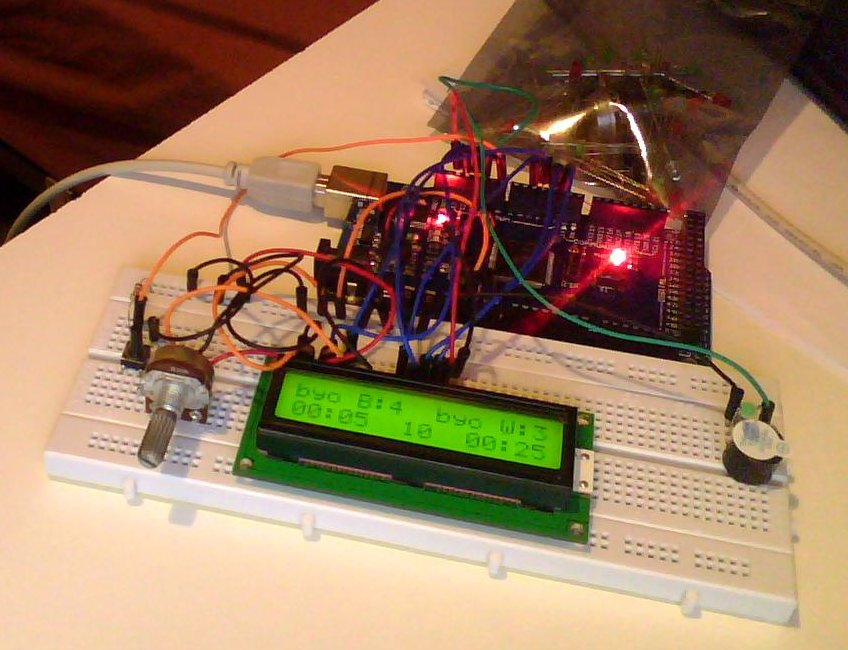
\includegraphics[scale=0.4]{reloj.jpg}

Esta forma fue eliminada al poco tiempo, pues una de nuestras ideas, es que el
jugador no tenga que preocuparse del programa, pues está concentrado jugando.
Además, los factores externos eran demasiados, pues pensamos en modificar los
relojes de tiempo, para qué el propio botón que indicaba al reloj el final del
tiempo, fuese el mismo que nos indicase a nosotros el momento de tomar la foto.
Con todo esto, lo unico que podiamos conseguir es que nuestro programa no fuese
funcional, ya que nadie podria hacer uso de nuestro programa sin dicho reloj.
Tras pensar distintas formas de solucionar los problemas que daba dicha
implementación, decidimos cambiar por completo la idea.  


\subsection{2ª Implementación: detección por diferencias sin turnos}

En esta segunda implementación pensamos en suprimir el uso de botones y
decidimos buscar la diferencia de cada imagen con la anteior, buscando círculos
en esa diferencia. Esta solución nos pareció mucho mejor que la anterior, pero
empezamos a darnos cuenta que detectaba toda la trayectoria que hacia la piedra
hasta estar colocada en su sitio, haciendo que el programa nos detectase piedras
donde realmente no se habian puesto, esto se podria haber solucionado
estadísticamente, pero esto lo descubrimos más tarde, asi que en ese momento se
descartó esta idea y enfocamos la solución de otra forma. Además, el hacer la
diferencia de todas las imágenes conllevaba un coste de procesamiento a tener en
cuenta, al cual había que añadirle la búsqueda de círculos, suma que es
demasiado elevada y creaba un tiempo de retreso que se iba acumulando, haciendo
que en determinado momento fallase el programa.

\subsection{3ª Implementación: detección por circuferencias y estadística}

Y como dice el refrán, a la tercera va la vencida. Esta vez, ya teniamos más
experiencia y el tablero ya estaba idealizado. Por esto, pensamos que la mejor
solución podría ser la más sencilla, para ello, sin hacer tratamiento ni
diferencias, buscamos círculos en la imagen ideal. Con una matriz de estadística
temporal, vamos buscando si los círculos se quedan de forma estable en una
posición, y en tal caso, podemos asegurar que la piedra esta colocada en ese
lugar, esta solución, ademas, permite llevar bien la cuenta de los turnos y el
momento en el que se puso la piedra, pues aunque tenga que pasar un tiempo para
asegurar que está la piedra, sabemos el momento en el que se puso. Además el
coste de ejecución es asumible.

Hemos detectado después de varias ejecuciones que cuando tenemos en el tablero
una cantidad de piedras muy grande, se comienza a utilizar mucho procesador,
pero no sabemos exactamente porque y tenemos que investigar un poco más. 

\subsection{Buscando colores}

Como en cada parte del proyecto, esta también ha tenido su evolución desde que
empezamos a plantearlo hasta el resultado final, mucho más pulido y funcional.
En un principio y dado que los jugadores nos iban a ir marcando el ritmo de
turnos, simplemente deberíamos de saber si le tocaba colocar a blancas o negras, como
siempre empiezan negras, por reglas del propio juego, sólo deberíamos de detectar la
piedra que se colocaba y automáticamente obtendríamos el color. 
Debido a que esto cambió a lo largo del tiempo y en la actualidad la forma de
encontrar piedras es distinta, debemos saber de que color es la piedra que se ha
detectado en cada momento, para ello una vez que detectamos una piedra, debemos
asegurarnos de que color es. La forma de hacerlo es buscando en el punto central
donde esta situada la piedra e ir a su pixel y analizar el color. Gracias a
OpenCv esta labor es relativamente sencilla, pero nos dimos cuenta, debido a la
calidad de las imágenes, que no todo iba a ser color de rosa. El gran problema
que tenemos es que las piedras al ser redondeadas, la cámara capta reflejos de
dichas piedras haciendo que el color de las piedras pueda llegar a confundirse
fácilmente si no cogen un número amplio de muestras para saber el color. Aun
asi, los test dan fallos a veces, para evitar esto, tenemos que variar un umbral
para el color blanco, el cual tenemos pensado en un futuro que se detecte
automáticamente de alguna forma.

%
% API Documentation for API Documentation
% Módulo src.search_stones
%
% Generated by epydoc 3.0.1
% [Wed Sep 12 04:59:27 2012]
%

%%%%%%%%%%%%%%%%%%%%%%%%%%%%%%%%%%%%%%%%%%%%%%%%%%%%%%%%%%%%%%%%%%%%%%%%%%%
%%                          Módulo Descripción                           %%
%%%%%%%%%%%%%%%%%%%%%%%%%%%%%%%%%%%%%%%%%%%%%%%%%%%%%%%%%%%%%%%%%%%%%%%%%%%

    \index{src \textit{(package)}!src.search\_stones \textit{(module)}|(}
\section{Módulo src.search\_stones}

    \label{src:search_stones}

%%%%%%%%%%%%%%%%%%%%%%%%%%%%%%%%%%%%%%%%%%%%%%%%%%%%%%%%%%%%%%%%%%%%%%%%%%%
%%                               Funciones                               %%
%%%%%%%%%%%%%%%%%%%%%%%%%%%%%%%%%%%%%%%%%%%%%%%%%%%%%%%%%%%%%%%%%%%%%%%%%%%

  \subsection{Funciones}

    \label{src:search_stones:search_stones}
    \index{src \textit{(package)}!src.search\_stones \textit{(module)}!src.search\_stones.search\_stones \textit{(function)}}

    \vspace{0.5ex}

\hspace{.8\funcindent}\begin{boxedminipage}{\funcwidth}

    \raggedright \textbf{search\_stones}(\textit{img}, \textit{corners}, \textit{dp}={\tt 1.7})

    \vspace{-1.5ex}

    \rule{\textwidth}{0.5\fboxrule}
\setlength{\parskip}{2ex}
Devuelve las circunferencias encontradas en una imagen.

\setlength{\parskip}{1ex}
      \textbf{Parámetros}
      \vspace{-1ex}

      \begin{quote}
        \begin{Ventry}{xxxxxxx}

          \item[img]


imagen donde buscaremos las circunferencias
            {\it (tipo=IplImage)}

          \item[corners]


lista de esquinas
            {\it (tipo=list)}

          \item[dp]


profundidad de búsqueda de círculos
            {\it (tipo=int)}

          \item[dp]


1.7 era el valor que mejor funcionaba. Prueba y error
            {\it (tipo=int)}

        \end{Ventry}

      \end{quote}

    \end{boxedminipage}

    \label{src:search_stones:check_color_stone}
    \index{src \textit{(package)}!src.search\_stones \textit{(module)}!src.search\_stones.check\_color\_stone \textit{(function)}}

    \vspace{0.5ex}

\hspace{.8\funcindent}\begin{boxedminipage}{\funcwidth}

    \raggedright \textbf{check\_color\_stone}(\textit{pt}, \textit{radious}, \textit{img}, \textit{threshold}={\tt 190})

    \vspace{-1.5ex}

    \rule{\textwidth}{0.5\fboxrule}
\setlength{\parskip}{2ex}
Devuelve el color de la piedra dado el centro y el radio de la piedra y una imagen. También desechamos las piedras que no sean negras o blancas.

\setlength{\parskip}{1ex}
      \textbf{Parámetros}
      \vspace{-1ex}

      \begin{quote}
        \begin{Ventry}{xxxxxxxxx}

          \item[pt]


centro de la piedra
            {\it (tipo=tuple)}

          \item[radious]


radio de la piedra
            {\it (tipo=int)}

          \item[img]


imagen donde comprobaremos el color de ciertos pixeles
            {\it (tipo=IplImage)}

          \item[threshold]


umbral de blanco
            {\it (tipo=int)}

          \item[threshold]


190 cuando hay buena luminosidad
            {\it (tipo=int)}

        \end{Ventry}

      \end{quote}

    \end{boxedminipage}


%%%%%%%%%%%%%%%%%%%%%%%%%%%%%%%%%%%%%%%%%%%%%%%%%%%%%%%%%%%%%%%%%%%%%%%%%%%
%%                               Variables                               %%
%%%%%%%%%%%%%%%%%%%%%%%%%%%%%%%%%%%%%%%%%%%%%%%%%%%%%%%%%%%%%%%%%%%%%%%%%%%

  \subsection{Variables}

    \vspace{-1cm}
\hspace{\varindent}\begin{longtable}{|p{\varnamewidth}|p{\vardescrwidth}|l}
\cline{1-2}
\cline{1-2} \centering \textbf{Nombre} & \centering \textbf{Descripción}& \\
\cline{1-2}
\endhead\cline{1-2}\multicolumn{3}{r}{\small\textit{continúa en la página siguiente}}\\\endfoot\cline{1-2}
\endlastfoot\raggedright \_\-\_\-p\-a\-c\-k\-a\-g\-e\-\_\-\_\- & \raggedright \textbf{Valor:} 
{\tt \texttt{'}\texttt{src}\texttt{'}}&\\
\cline{1-2}
\end{longtable}

    \index{src \textit{(package)}!src.search\_stones \textit{(module)}|)}


%
% API Documentation for API Documentation
% Module src.stone
%
% Generated by epydoc 3.0.1
% [Wed Sep 12 02:49:43 2012]
%

%%%%%%%%%%%%%%%%%%%%%%%%%%%%%%%%%%%%%%%%%%%%%%%%%%%%%%%%%%%%%%%%%%%%%%%%%%%
%%                          Module Description                           %%
%%%%%%%%%%%%%%%%%%%%%%%%%%%%%%%%%%%%%%%%%%%%%%%%%%%%%%%%%%%%%%%%%%%%%%%%%%%

    \index{src \textit{(package)}!src.stone \textit{(module)}|(}
\section{Module src.stone}

    \label{src:stone}

%%%%%%%%%%%%%%%%%%%%%%%%%%%%%%%%%%%%%%%%%%%%%%%%%%%%%%%%%%%%%%%%%%%%%%%%%%%
%%                               Variables                               %%
%%%%%%%%%%%%%%%%%%%%%%%%%%%%%%%%%%%%%%%%%%%%%%%%%%%%%%%%%%%%%%%%%%%%%%%%%%%

  \subsection{Variables}

    \vspace{-1cm}
\hspace{\varindent}\begin{longtable}{|p{\varnamewidth}|p{\vardescrwidth}|l}
\cline{1-2}
\cline{1-2} \centering \textbf{Name} & \centering \textbf{Description}& \\
\cline{1-2}
\endhead\cline{1-2}\multicolumn{3}{r}{\small\textit{continued on next page}}\\\endfoot\cline{1-2}
\endlastfoot\raggedright \_\-\_\-p\-a\-c\-k\-a\-g\-e\-\_\-\_\- & \raggedright \textbf{Value:} 
{\tt \texttt{'}\texttt{src}\texttt{'}}&\\
\cline{1-2}
\raggedright c\-o\-l\-o\-r\- & \raggedright color de la piedra

            {\it (type=int)}&\\
\cline{1-2}
\raggedright i\-m\-g\- & \raggedright imagen donde se encuentra la piedra

            {\it (type=IplImage)}&\\
\cline{1-2}
\raggedright p\-i\-x\- & \raggedright pixel donde se encuentra la piedra dentro de la imagen

            {\it (type=tuple)}&\\
\cline{1-2}
\raggedright p\-t\- & \raggedright coordenada del tablero donde se encuentra la piedra

            {\it (type=tuple)}&\\
\cline{1-2}
\raggedright x\- & \raggedright coordenada x del tablero donde se encuentra la piedra

            {\it (type=int)}&\\
\cline{1-2}
\raggedright y\- & \raggedright coordenada y del tablero donde se encuentra la piedra

            {\it (type=int)}&\\
\cline{1-2}
\end{longtable}


%%%%%%%%%%%%%%%%%%%%%%%%%%%%%%%%%%%%%%%%%%%%%%%%%%%%%%%%%%%%%%%%%%%%%%%%%%%
%%                           Class Description                           %%
%%%%%%%%%%%%%%%%%%%%%%%%%%%%%%%%%%%%%%%%%%%%%%%%%%%%%%%%%%%%%%%%%%%%%%%%%%%

    \index{src \textit{(package)}!src.stone \textit{(module)}!src.stone.Stone \textit{(class)}|(}
\subsection{Class Stone}

    \label{src:stone:Stone}

Clase piedra.

%%%%%%%%%%%%%%%%%%%%%%%%%%%%%%%%%%%%%%%%%%%%%%%%%%%%%%%%%%%%%%%%%%%%%%%%%%%
%%                                Methods                                %%
%%%%%%%%%%%%%%%%%%%%%%%%%%%%%%%%%%%%%%%%%%%%%%%%%%%%%%%%%%%%%%%%%%%%%%%%%%%

  \subsubsection{Methods}

    \label{src:stone:Stone:__init__}
    \index{src \textit{(package)}!src.stone \textit{(module)}!src.stone.Stone \textit{(class)}!src.stone.Stone.\_\_init\_\_ \textit{(method)}}

    \vspace{0.5ex}

\hspace{.8\funcindent}\begin{boxedminipage}{\funcwidth}

    \raggedright \textbf{\_\_init\_\_}(\textit{self}, \textit{color}, \textit{img}={\tt None}, \textit{pix}={\tt None}, \textit{pt}={\tt None})

    \vspace{-1.5ex}

    \rule{\textwidth}{0.5\fboxrule}
\setlength{\parskip}{2ex}

Inicializamos una piedra, si no tenemos la posición, buscamos cual
es esa posición dado una imagen ideal y un pixel.
:param color: color de la piedra, BLACK or WHITE
:type color: int
:param img: imagen en formato ideal
:type img: IplImage
:keyword img: None si no le pasamos ninguna imagen por parámetro
:param pix: pixel donde se encuentra la piedra en la imagen
:type pix: tuple
:keyword pix: None si no le pasamos ningun pixel por parámetro
:param pt: punto donde se encuentra la piedra en el tablero
:type pt: tuple
:keyword pt: None si no le pasamos ningún punto parámetro.
\setlength{\parskip}{1ex}
    \end{boxedminipage}

    \label{src:stone:Stone:__str__}
    \index{src \textit{(package)}!src.stone \textit{(module)}!src.stone.Stone \textit{(class)}!src.stone.Stone.\_\_str\_\_ \textit{(method)}}

    \vspace{0.5ex}

\hspace{.8\funcindent}\begin{boxedminipage}{\funcwidth}

    \raggedright \textbf{\_\_str\_\_}(\textit{self})

\setlength{\parskip}{2ex}
\setlength{\parskip}{1ex}
    \end{boxedminipage}

    \label{src:stone:Stone:__eq__}
    \index{src \textit{(package)}!src.stone \textit{(module)}!src.stone.Stone \textit{(class)}!src.stone.Stone.\_\_eq\_\_ \textit{(method)}}

    \vspace{0.5ex}

\hspace{.8\funcindent}\begin{boxedminipage}{\funcwidth}

    \raggedright \textbf{\_\_eq\_\_}(\textit{self}, \textit{st})

\setlength{\parskip}{2ex}
\setlength{\parskip}{1ex}
    \end{boxedminipage}

    \label{src:stone:Stone:__cmp__}
    \index{src \textit{(package)}!src.stone \textit{(module)}!src.stone.Stone \textit{(class)}!src.stone.Stone.\_\_cmp\_\_ \textit{(method)}}

    \vspace{0.5ex}

\hspace{.8\funcindent}\begin{boxedminipage}{\funcwidth}

    \raggedright \textbf{\_\_cmp\_\_}(\textit{self}, \textit{st})

\setlength{\parskip}{2ex}
\setlength{\parskip}{1ex}
    \end{boxedminipage}

    \label{src:stone:Stone:__hash__}
    \index{src \textit{(package)}!src.stone \textit{(module)}!src.stone.Stone \textit{(class)}!src.stone.Stone.\_\_hash\_\_ \textit{(method)}}

    \vspace{0.5ex}

\hspace{.8\funcindent}\begin{boxedminipage}{\funcwidth}

    \raggedright \textbf{\_\_hash\_\_}(\textit{self})

\setlength{\parskip}{2ex}
\setlength{\parskip}{1ex}
    \end{boxedminipage}

    \index{src \textit{(package)}!src.stone \textit{(module)}!src.stone.Stone \textit{(class)}|)}
    \index{src \textit{(package)}!src.stone \textit{(module)}|)}


\section{Conexión con el servidor}

Para la conexión al servidor comenzamos intentándolo con los servidores de KGS,
pero la falta de documentación de protocolos de dicho servidor y el tener un
protocolo cerrado hizo imposible esta tarea. Aun así, queremos hacer posible la
conexión a este servidor, pues es de los más usados. Actualmente el programa se
conecta a IGS a traves de un usuario registrado siguiendo el protocolo de dicho
servidorl, que es libre.

Para el intento de conexión con el servidor de KGS hemos contactado con algunos
administradores de KGS, pero finalmente nos han dicho que no puede ofrecernos
ninguna API o programa para facilitarnos la subida de una partida, ya que el
protocolo es cerrado. 

%
% API Documentation for API Documentation
% Módulo src.igs
%
% Generated by epydoc 3.0.1
% [Wed Sep 12 04:59:27 2012]
%

%%%%%%%%%%%%%%%%%%%%%%%%%%%%%%%%%%%%%%%%%%%%%%%%%%%%%%%%%%%%%%%%%%%%%%%%%%%
%%                          Módulo Descripción                           %%
%%%%%%%%%%%%%%%%%%%%%%%%%%%%%%%%%%%%%%%%%%%%%%%%%%%%%%%%%%%%%%%%%%%%%%%%%%%

    \index{src \textit{(package)}!src.igs \textit{(module)}|(}
\section{Módulo src.igs}

    \label{src:igs}

%%%%%%%%%%%%%%%%%%%%%%%%%%%%%%%%%%%%%%%%%%%%%%%%%%%%%%%%%%%%%%%%%%%%%%%%%%%
%%                               Variables                               %%
%%%%%%%%%%%%%%%%%%%%%%%%%%%%%%%%%%%%%%%%%%%%%%%%%%%%%%%%%%%%%%%%%%%%%%%%%%%

  \subsection{Variables}

    \vspace{-1cm}
\hspace{\varindent}\begin{longtable}{|p{\varnamewidth}|p{\vardescrwidth}|l}
\cline{1-2}
\cline{1-2} \centering \textbf{Nombre} & \centering \textbf{Descripción}& \\
\cline{1-2}
\endhead\cline{1-2}\multicolumn{3}{r}{\small\textit{continúa en la página siguiente}}\\\endfoot\cline{1-2}
\endlastfoot\raggedright \_\-\_\-p\-a\-c\-k\-a\-g\-e\-\_\-\_\- & \raggedright \textbf{Valor:} 
{\tt \texttt{'}\texttt{src}\texttt{'}}&\\
\cline{1-2}
\raggedright p\-w\-d\- & \raggedright password correspondiente al usuario de Igs

            {\it (tipo=str)}&\\
\cline{1-2}
\raggedright s\- & \raggedright socket para la conexión con el servidor

            {\it (tipo=socket)}&\\
\cline{1-2}
\raggedright u\-s\-e\-r\- & \raggedright usuario del servidor Igs

            {\it (tipo=str)}&\\
\cline{1-2}
\end{longtable}


%%%%%%%%%%%%%%%%%%%%%%%%%%%%%%%%%%%%%%%%%%%%%%%%%%%%%%%%%%%%%%%%%%%%%%%%%%%
%%                           Clase Descripción                           %%
%%%%%%%%%%%%%%%%%%%%%%%%%%%%%%%%%%%%%%%%%%%%%%%%%%%%%%%%%%%%%%%%%%%%%%%%%%%

    \index{src \textit{(package)}!src.igs \textit{(module)}!src.igs.Igs \textit{(class)}|(}
\subsection{Clase Igs}

    \label{src:igs:Igs}

Clase que se comunica con el servidor de IGS.

%%%%%%%%%%%%%%%%%%%%%%%%%%%%%%%%%%%%%%%%%%%%%%%%%%%%%%%%%%%%%%%%%%%%%%%%%%%
%%                                Métodos                                %%
%%%%%%%%%%%%%%%%%%%%%%%%%%%%%%%%%%%%%%%%%%%%%%%%%%%%%%%%%%%%%%%%%%%%%%%%%%%

  \subsubsection{Métodos}

    \label{src:igs:Igs:__init__}
    \index{src \textit{(package)}!src.igs \textit{(module)}!src.igs.Igs \textit{(class)}!src.igs.Igs.\_\_init\_\_ \textit{(method)}}

    \vspace{0.5ex}

\hspace{.8\funcindent}\begin{boxedminipage}{\funcwidth}

    \raggedright \textbf{\_\_init\_\_}(\textit{self}, \textit{user}={\tt \texttt{'}\texttt{rocamgo}\texttt{'}}, \textit{pwd}={\tt \texttt{'}\texttt{qwe}\texttt{'}})

    \vspace{-1.5ex}

    \rule{\textwidth}{0.5\fboxrule}
\setlength{\parskip}{2ex}
Inicializamos la conexión con el servidor y creamos un tablero de aprendizaje dentro del servidor para comenzar a subir la partida.

\setlength{\parskip}{1ex}
      \textbf{Parámetros}
      \vspace{-1ex}

      \begin{quote}
        \begin{Ventry}{xxxx}

          \item[user]


usuario que se conectará al servidor
            {\it (tipo=str)}

          \item[pwd]


contraseña del usuario para conetarse al servidor
            {\it (tipo=str)}

        \end{Ventry}

      \end{quote}

    \end{boxedminipage}

    \label{src:igs:Igs:add_stone}
    \index{src \textit{(package)}!src.igs \textit{(module)}!src.igs.Igs \textit{(class)}!src.igs.Igs.add\_stone \textit{(method)}}

    \vspace{0.5ex}

\hspace{.8\funcindent}\begin{boxedminipage}{\funcwidth}

    \raggedright \textbf{add\_stone}(\textit{self}, \textit{pos})

    \vspace{-1.5ex}

    \rule{\textwidth}{0.5\fboxrule}
\setlength{\parskip}{2ex}
Añadimos piedra al servidor.

\setlength{\parskip}{1ex}
      \textbf{Parámetros}
      \vspace{-1ex}

      \begin{quote}
        \begin{Ventry}{xxx}

          \item[pos]


posición de la piedra a añadir
            {\it (tipo=tuple)}

        \end{Ventry}

      \end{quote}

    \end{boxedminipage}

    \label{src:igs:Igs:close}
    \index{src \textit{(package)}!src.igs \textit{(module)}!src.igs.Igs \textit{(class)}!src.igs.Igs.close \textit{(method)}}

    \vspace{0.5ex}

\hspace{.8\funcindent}\begin{boxedminipage}{\funcwidth}

    \raggedright \textbf{close}(\textit{self})

    \vspace{-1.5ex}

    \rule{\textwidth}{0.5\fboxrule}
\setlength{\parskip}{2ex}
Cerramos la conexión con el servidor.

\setlength{\parskip}{1ex}
    \end{boxedminipage}

    \index{src \textit{(package)}!src.igs \textit{(module)}!src.igs.Igs \textit{(class)}|)}
    \index{src \textit{(package)}!src.igs \textit{(module)}|)}


\section{Creación del archivo .sgf}

Para la creación del archivo .sgf no tuvimos muchos problemas ya que es un
archivo de texto que esta estandarizado y sigue una reglas fáciles de seguir.
Solo hemos tenido como trabajar con ficheros en python y escribir unas líneas de
código para conseguir lo deseado.

Desctacar que en el servidor IGS, una de las letras se la sala, y tenemos que
cambiar el sistema de nombramiento para subir una partida a IGS, del sistema de
nombramiento que usamos para guardar el sgf. 

%
% API Documentation for API Documentation
% Module src.kifu
%
% Generated by epydoc 3.0.1
% [Sun Sep  9 21:09:35 2012]
%

%%%%%%%%%%%%%%%%%%%%%%%%%%%%%%%%%%%%%%%%%%%%%%%%%%%%%%%%%%%%%%%%%%%%%%%%%%%
%%                          Module Description                           %%
%%%%%%%%%%%%%%%%%%%%%%%%%%%%%%%%%%%%%%%%%%%%%%%%%%%%%%%%%%%%%%%%%%%%%%%%%%%

    \index{src \textit{(package)}!src.kifu \textit{(module)}|(}
\section{Module src.kifu}

    \label{src:kifu}

%%%%%%%%%%%%%%%%%%%%%%%%%%%%%%%%%%%%%%%%%%%%%%%%%%%%%%%%%%%%%%%%%%%%%%%%%%%
%%                               Variables                               %%
%%%%%%%%%%%%%%%%%%%%%%%%%%%%%%%%%%%%%%%%%%%%%%%%%%%%%%%%%%%%%%%%%%%%%%%%%%%

  \subsection{Variables}

    \vspace{-1cm}
\hspace{\varindent}\begin{longtable}{|p{\varnamewidth}|p{\vardescrwidth}|l}
\cline{1-2}
\cline{1-2} \centering \textbf{Name} & \centering \textbf{Description}& \\
\cline{1-2}
\endhead\cline{1-2}\multicolumn{3}{r}{\small\textit{continued on next page}}\\\endfoot\cline{1-2}
\endlastfoot\raggedright \_\-\_\-p\-a\-c\-k\-a\-g\-e\-\_\-\_\- & \raggedright \textbf{Value:} 
{\tt \texttt{'}\texttt{src}\texttt{'}}&\\
\cline{1-2}
\end{longtable}


%%%%%%%%%%%%%%%%%%%%%%%%%%%%%%%%%%%%%%%%%%%%%%%%%%%%%%%%%%%%%%%%%%%%%%%%%%%
%%                           Class Description                           %%
%%%%%%%%%%%%%%%%%%%%%%%%%%%%%%%%%%%%%%%%%%%%%%%%%%%%%%%%%%%%%%%%%%%%%%%%%%%

    \index{src \textit{(package)}!src.kifu \textit{(module)}!src.kifu.Kifu \textit{(class)}|(}
\subsection{Class Kifu}

    \label{src:kifu:Kifu}
Clase para crear un fichero .sgf y guardar la partida.


%%%%%%%%%%%%%%%%%%%%%%%%%%%%%%%%%%%%%%%%%%%%%%%%%%%%%%%%%%%%%%%%%%%%%%%%%%%
%%                                Methods                                %%
%%%%%%%%%%%%%%%%%%%%%%%%%%%%%%%%%%%%%%%%%%%%%%%%%%%%%%%%%%%%%%%%%%%%%%%%%%%

  \subsubsection{Methods}

    \label{src:kifu:Kifu:__init__}
    \index{src \textit{(package)}!src.kifu \textit{(module)}!src.kifu.Kifu \textit{(class)}!src.kifu.Kifu.\_\_init\_\_ \textit{(method)}}

    \vspace{0.5ex}

\hspace{.8\funcindent}\begin{boxedminipage}{\funcwidth}

    \raggedright \textbf{\_\_init\_\_}(\textit{self}, \textit{player1}={\tt \texttt{'}\texttt{j1}\texttt{'}}, \textit{player2}={\tt \texttt{'}\texttt{j2}\texttt{'}}, \textit{handicap}={\tt 0}, \textit{path}={\tt \texttt{'}\texttt{sgf}\texttt{'}}, \textit{rank\_player1}={\tt \texttt{'}\texttt{20k}\texttt{'}}, \textit{rank\_player2}={\tt \texttt{'}\texttt{20k}\texttt{'}})

    \vspace{-1.5ex}

    \rule{\textwidth}{0.5\fboxrule}
\setlength{\parskip}{2ex}
    Inicializamos configuración del archivo sgf. :param  player1: nombre 
    del jugador 1 :type  player1: str :keyword  player1: j1 por defecto 
    :param  player2: nombre del jugador 2 :type  player2: str :keyword  
    player2: j2 por defecto :param  handicap: handicap dado en la partida 
    :type  handicap: int :keyword  handicap: ninguno por defecto (0) :param
    path: ruta relativa donde guardamos el fichero :type  path: str 
    :keyword  path: carpeta sgf por defecto :param  rank\_player1: rango 
    del jugador 1 :type  rank\_player1: str :keyword  rank\_player1: 20k 
    por defecto, nivel de inicio en el go :param  rank\_player2: rango del 
    jugador 2 :type  rank\_player2: str :keyword  rank\_player2: 20k por 
    defecto, nivel de inicio en el go

\setlength{\parskip}{1ex}
    \end{boxedminipage}

    \label{src:kifu:Kifu:add_stone}
    \index{src \textit{(package)}!src.kifu \textit{(module)}!src.kifu.Kifu \textit{(class)}!src.kifu.Kifu.add\_stone \textit{(method)}}

    \vspace{0.5ex}

\hspace{.8\funcindent}\begin{boxedminipage}{\funcwidth}

    \raggedright \textbf{add\_stone}(\textit{self}, \textit{pos}, \textit{color})

    \vspace{-1.5ex}

    \rule{\textwidth}{0.5\fboxrule}
\setlength{\parskip}{2ex}
    Añadir piedra al sgf. :param pos: posición de la piedra :type pos: 
    tuple :param color: color de la piedra :type color: int

\setlength{\parskip}{1ex}
    \end{boxedminipage}

    \label{src:kifu:Kifu:end_file}
    \index{src \textit{(package)}!src.kifu \textit{(module)}!src.kifu.Kifu \textit{(class)}!src.kifu.Kifu.end\_file \textit{(method)}}

    \vspace{0.5ex}

\hspace{.8\funcindent}\begin{boxedminipage}{\funcwidth}

    \raggedright \textbf{end\_file}(\textit{self})

    \vspace{-1.5ex}

    \rule{\textwidth}{0.5\fboxrule}
\setlength{\parskip}{2ex}
    Cerrar el fichero y dejarlo listo para poder abrirlo.

\setlength{\parskip}{1ex}
    \end{boxedminipage}

    \index{src \textit{(package)}!src.kifu \textit{(module)}!src.kifu.Kifu \textit{(class)}|)}
    \index{src \textit{(package)}!src.kifu \textit{(module)}|)}


\chapter{Diagrama de gant}

A continuación vemos el diagrama de gant, con la explicación de las horas aproximadas invertidas por cada uno.

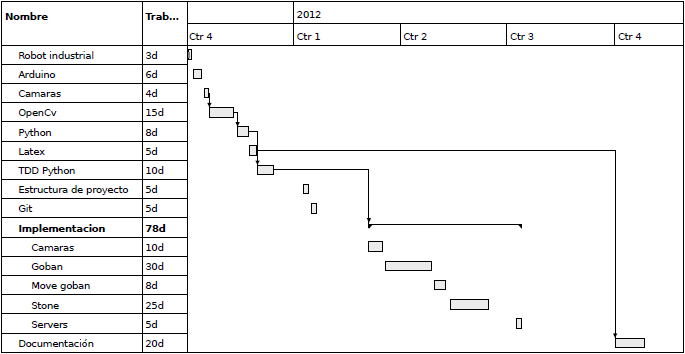
\includegraphics[scale=0.9]{gant.png}\\

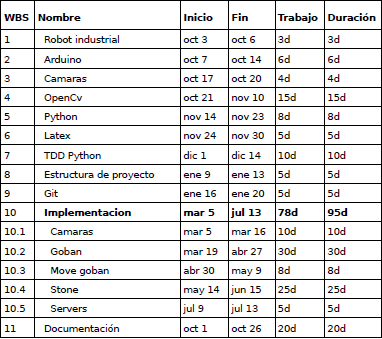
\includegraphics[scale=1.4]{gant2.png}

\chapter{Manual de usuario}

\section{Guía de instalación} 

Para la instalación del proyecto, al menos de lo que se encuentra activo
actualmente, porque como hemos comentado, el proyecto no está terminado, pero
podremos ver los últimos cambios utilizando la última versión disponible en
GitHub del proyecto. Este proyecto se ha probado solamente en Linux, aunque
debería de funcionar en otros Sistemas Operativos, ya que se ha programado
con esa intención.

Para que funcione el proyecto, necesitaremos instalar unas cuantas de bibliotecas
que hemos usado: OpenCv, unittest, nosetest y numpy.

Para su instalación, ejecutamos el siguiente comando:

\begin{verbatim}
sudo apt-get install python-unittest2 python-OpenCv python-nose python-numpy
\end{verbatim}

Comenzamos descargándonos el proyecto desde GitHub, para ello necesitaremos
tener instalado git, que en las distribuciones de Linux basadas en debian,
podemos instalarlo de la siguiente manera: 

\begin{verbatim}
sudo apt-get install git
\end{verbatim}

Ejecutamos el siguiente comando para descargarnos el proyecto: 

\begin{verbatim}
git clone git@github.com:Virako/Rocamgo.git
\end{verbatim}

Dentro de esta carpeta nos encontraremos con los últimos cambios realizados en
el proyecto.


\section{Cómo utilizarlo}

Para hacerlo funcionar deberemos ejecutar desde la carpeta raiz,
que se llamará Rocamgo si no se ha cambiado, el siguiente comando:

\begin{verbatim}
python src/rocamgo.py
\end{verbatim}

Este comando nos devolverá la ayuda para ejecutar el programa utilizando una
webcam o un video pasándole la ruta.

Si seleccionamos la \textbf{''webcam''}, nos dará a elegir entre las webcam que tengamos, o
si solo tenemos una, la selecciona por defecto.

Antes de ejecutar el proyecto, debemos asegurarnos que tenemos preparado el
terreno de juego, para ello necesitamos que el tablero este colocado en una
superficie lo más lisa posible y la cámara conectada al PC donde se ejecutará
el programa, a poder ser de una buena calidad, apuntando al tablero donde se
jugará la partida.  Debemos intentar que la cámara enfoque correctamente al
tablero, centrando este dentro de la imagen lo máximo posible. El programa será
capaz de funcionar siempre y cuando en la imagen se vean correctamente todas
las partes del tablero.

En el caso de que tengamos más de una cámara conectada, nos mostrará ventanas
con las difrentes cámaras, para seleccionar la cámara que deseemos, pulsamos
doble click encima de la cámara deseada.

Si seleccionamos un \textbf{''video''}, pasamos directamente al siguiente paso. 

Luego, tanto si hemo seleccionado cámara como si hemos seleccionado video, nos
pedirá un nombre de usuario del servidor IGS.  Para crearnos un usuario en este
servidor, podemos registrarnos en la siguiente página:
\url{http://www.pandanet-igs.com/igs_users/register}


\section{Actualizaciones}

Para actualizaciones del proyecto, una vez lo hayamos descargado con git, solo
tenemos que entrar dentro del directorio y ejecutar git pull, el cual se
descargará los últimos cambios que haya en el servidor. 


\chapter{Conclusiones}

Como hemos comentado anteriormente en la implementación del proyecto, nos hemos
dado cuenta de que nuestros objetivos iniciales para este Proyecto Fin de
Carrera eran demasiado ambiciosos, por lo cual no hemos podido completar todos
los objetivos de cara al proyecto. Se ha conseguido realizar gran parte del
software que teniamos pensado, pero debido al coste, tanto temporal como
económico del brazo robótico, hemos dejado esta parte para una línea futura,
centrándonos principalmente en la captación de imágenes y su tratamiento.

Desde el principio de este proyecto, hemos estado aprendiendo bastante sobre las
bibliotecas de OpenCv, las cuales son una maravilla y nos han ayudado muchísimo en
la implementación de este proyecto. Creemos que todavía nos queda mucho que
aprender sobre estas bibliotecas, las cuales esperamos aprender más en un futuro. 

Cuando nos hemos ido adentrando en el proyecto, nos han ido surgiéndo muchísimos
problemas, sobre todo con la detección del tablero, ya que lo pensado y la
realidad, se han ido distanciando un poco. 

La utilización de git nos ha hecho aprender y abrirnos la mente al utilizar un
controlador de versiones distribuidos, a parte de servirnos de mucha ayuda al
ser un proyecto en grupo. 

La gran utilización de python nos ha hecho subir nuestro nivel de programación
en este lenguaje.

El usar filosofía TDD y hacer test en el proyecto nos han ayudado a realizar
algunas cosas más rápido y comprobar el correcto funcionamiento de algunas
funcionalidades, como por ejemplo, en la detección del tablero. Gracias a esto
conocimos también algunas herramientas como TravisCI, la cual puede sernos de
gran utilidad más adelante. 

La utilización de Latex, al estar acostumbrados a programar, no nos ha resultado
muy complicada. Cuando observamos como quedan los documentos, la verdad es que
nos ha fascinado, y tenemos pensamiento de utilizarlo para otros textos en un
futuro, es una herramienta que nos ha cautivado.

El conectarnos al servidor de IGS, nos ha hecho que aprendamos a utilizar un
poco los sockets.

Aunque finalmente no utilizamos arduino para los relojes, también nos llevamos
un tiempo manejandolos y aprendimos bastante, ya que usamos botones, pantalla
LCD, potenciómetros y buzzer.

Destacar a vim dentro de todos los editores de texto que hemos utilizado, ya que
aunque la curva de aprendizaje sea bastante dura, finalmente podemos decir que
la productividad aumenta. 

Agradecer a toda la comunidad del software libre de nuevo, por que gracias a
ella, hemos tenido un sistema operativo con un software bastante bueno para la
realización de todo el proyecto, así como el acceso a una gran cantidad de
código libre para ver ejemplos de como hacer las cosas, ya que creemos que la
mejor forma de aprender es con ejemplos. Sin dejar atrás las webs de preguntas y
respuestas, los foros y los chats, que nos han solucionado más de una duda. 



\chapter{Líneas futuras}

El futuro de este proyecto sigue día a día, y esperamos que poco a poco se vaya
mejorando hasta conseguir todos los objetivos deseados, aunque por temas de
tiempo o dinero, no hemos podido terminar para este Proyecto Fin de Carrera. 

Principalmente queremos seguir mejorando la detección de partida de cara al
siguiente torneo de go, para ver si podemos llegar a utilizarlo completamente
para una partida real, en la cual seguramente aprendamos mucho y encontremos
errores nuevos para poder mejorar, por que como ya nos hemos dado cuenta, la
realidad se aleja de lo pensado, cada sitio donde se situe el tablero o que
cámara se escoja, seguramente de nuevos fallos que tendremos que ir puliendo
poco a poco. Estamos deseando llevar el proyecto al siguiente torneo para ver si
le gusta a la gente y ver su funcionamento en distintos sitios, con distinta
luminosidad, distintos jugadores que mueban más o menos el tablero, se usen
tableros o piedras distintas, en tonalidad sobre todo. 

Otra de las cosas que ya decidimos a mitad del proyecto de descartar, es hacer
el brazo robótico, porque un brazo rápido y preciso costaba muy caro, en precio
o en tiempo. En un futuro tenemos pensado gastarnos ese dinero o tiempo para
crear el brazo, ya que es una cosa que nos entusiasma bastante. Las
funcionalidades que aportaría este brazo serían más posibilidades de juego,
entre las cuales se encuentra que personas invidentes puedan utilizar este
programa para jugar partidas pos Internet fácilmente, simplemente añadiéndole un
comando al brazo para qué espere a que la mano de la persona invidente lo toque,
para saber donde a puesto la piedra el brazo. 

Una cosa que actualmente tenemos pendiente y llevamos unas semana intercambiando
correos con los administradores es subir la partida a KGS, por que como el
protocolo es cerrado, necesitamos que nos hagan algún cliente o algo especial
para poderlo utilizar. Esperamos que un futuro no muy lejano, las partidas
puedan subirse a KGS al igual que lo hacemos en IGS. 

Otras de los objetivos del proyecto que no hemos podido realizar, es la
posibilidad de adaptar este proyecto para qué funciones en los móviles o en
ordenadores de bajo coste como la Raspberry Pi. Para ello, tenemos en mente hacer
que nuestro proyecto ejecute varios hilos, haciendo que el procesamiento de
imágenes sea lo menos pesado posible.


\chapter{Licencia}

\section{Licencia de este manual}

\textbf{Reconocimiento - CompartirIgual (by-sa):} Se permite el uso comercial de
la obra y de las posibles obras derivadas, la distribución de las cuales se debe
hacer con una licencia igual a la que regula la obra original. \\ \\

%\includegraphics[scale=5]{licencia.png} 

Autores: 
\begin{itemize} 
    \item David Medina Velasco. \textbf{Email:} cuidadoconeltecho at gmail dot
    com 
    \item Víctor Ramírez de la Corte. \textbf{Email:} virako.9 at gmail dot com 
\end{itemize}

\section{Licencia de Rocamgo}

This program is free software: you can redistribute it and/or modify it under
the terms of the GNU General Public License as published by the Free Software
Foundation, either version 3 of the License, or (at your option) any later
version. \\ \\ This program is distributed in the hope that it will be useful,
but WITHOUT ANY WARRANTY; without even the implied warranty of MERCHANTABILITY
or FITNESS FOR A PARTICULAR PURPOSE.  See the GNU General Public License for
more details. \\ \\ You should have received a copy of the GNU General Public
License along with this program.  If not, see \url{http://www.gnu.org/licenses/}



\chapter{Bibliografía}


\subsubsection{Python }

Test unitarios para Python.
\url{http://docs.python.org/library/unittest.html}

Guía de estilos de Python.
\url{http://mundogeek.net/traducciones/guia-estilo-python.htm}

Guía de documentación de codigo Python.
\url{http://mundogeek.net/archivos/2008/07/07/documentacion-en-python/}

Guía de test de Python.
\url{http://www.magmax.org/2011/11/09/python-pruebas-4.html}

También consultado el libro 'Python para todos', el cual nos ha servido de gran
ayuda.
\url{http://mundogeek.net/tutorial-python/}

\subsubsection{Vim}

Empezamos usando como bibliografia la propia del programa, ya que incluye
vimtutor, un tutorial basico sobre el manejo de Vim.

Mas tarde comenzamos a practicar en la siguiente pagina.
\url{http://vimgolf.com/}

\subsubsection{Sobre brazos}

Diseño de un brazo mecánico.
\url{http://bit.ly/Qy6NOR}

Brazo robótico con GNU  Linux.
\url{http://www.linuxoriente.edu.sv/index.php?readmore=84}

Brazo robótico por 55 dolares.
\url{http://bit.ly/pLGrl6}

Tutorial para contruir el robot de 55 dolares.
\url{http://www.aonsquared.co.uk/robot_arm_tutorial_1}

Video de proyecto parecido.
\url{http://www.youtube.com/watch?v=lJehPbpA7AM}

Video de otro posible brazo.
\url{http://www.youtube.com/watch?v=d2OBCpbCEc4&feature=player_embedded}

Página de venta de servos.
\url{http://www.superrobotica.com/servos.htm}


\subsubsection{Internet Go Server (IGS)}

\url{http://gnugos60.blogspot.com/2007/04/internet-go-protocols.html}

\subsubsection{Go Text Protocol (GTP)}

Documentación del protocolo GTP v2.
\url{http://www.lysator.liu.se/~gunnar/gtp/gtp2-spec-draft2/gtp2-spec.html}

\subsubsection{GNU Go}

Código.
\url{http://ftp.gnu.org/gnu/gnugo/}

Documentación.
\url{http://www.gnu.org/software/gnugo/gnugo_toc.html}

\subsubsection{Proyecto parecido. Kifu}

\url{http://wiki.elphel.com/index.php?title=Kifu:_Go_game_record_(kifu)_generator}

\subsubsection{Pasar el tablero a modelo ideal}

\url{http://is.gd/k9k2K}

\subsubsection{Haartraining}

Detección rápida de objetos.
\url{http://note.sonots.com/SciSoftware/haartraining.html}

Referencia 5 del documento anterior.
\url{https://docs.google.com/View?docID=drw35kw_6gr8r84fs}

Programa prueba con codigo
\url{http://www.codeproject.com/KB/audio-video/haar_detection.aspx}

Explicación.
\url{http://www.coplec.org/?q=2010/08/05/entrenar-OpenCv}

\subsubsection{Enlaces interesantes sobre detección de objetos}

\url{http://en.wikipedia.org/wiki/SURF}

\url{http://en.wikipedia.org/wiki/Object_recognition_(computer_vision)}

\url{http://en.wikipedia.org/wiki/Template_matching}

\url{http://en.wikipedia.org/wiki/Pattern_recognition}

\url{http://www.pigeon.psy.tufts.edu/avc/kirkpatrick/}

\subsubsection{Proyecto interesante. Utilizando un proyector.}

\url{http://www.youtube.com/watch?feature=player_embedded&v=33Iyr16yhJQ}

\subsubsection{Para comandos de git.}
\url{http://alejandroandres.com/blog/2011/06/mi-workflow-con-git/}

\subsubsection{Guía de accesibilidad.}
\url{http://www.sidar.org/recur/direc/norm/index.php}

\subsubsection{Opencv.}
\url{http://OpenCv.willowgarage.com/}

\chapter{Apéndice A: ¿Qué es el go?} 

\url{http://es.wikipedia.org/wiki/Go}


\end{document}
